% !TEX program = xelatex
\documentclass[12pt,a4paper]{report}

% =========================
% MDUM8010 Dissertation Draft
% Generated from presentation notes.
% Compile with: xelatex -> biber -> xelatex -> xelatex
% =========================

\usepackage[a4paper,left=25mm,right=25mm,top=25mm,bottom=25mm]{geometry}
\usepackage{setspace}
\usepackage{fontspec}
\usepackage{graphicx}
\graphicspath{{figures/}}
\usepackage{booktabs}
\usepackage{array}
\usepackage{longtable}
\usepackage{tabularx}
\usepackage{multirow}
\usepackage{pdflscape}
\usepackage{float}
\usepackage{caption}
\usepackage{subcaption}
\usepackage{amsmath,amssymb}
\usepackage{enumitem}
\usepackage{xcolor}
\usepackage{hyperref}
\usepackage[backend=biber,style=authoryear,sorting=nyt,maxcitenames=2,maxbibnames=99]{biblatex}
\addbibresource{references.bib}

\setmainfont{Times New Roman}
\setsansfont{Arial}
\onehalfspacing
\setlength{\parindent}{2em}
\setlength{\parskip}{0.25em}

\hypersetup{
  colorlinks=true,
  linkcolor=black,
  citecolor=black,
  urlcolor=blue
}

\newcommand{\todo}[1]{\par\noindent\colorbox{yellow!25}{\parbox{0.96\linewidth}{\textbf{TODO:} #1}}\par}
\newcommand{\placeholderfig}[2]{%
\begin{figure}[H]
\centering
\fbox{\parbox[c][0.28\textheight][c]{0.88\linewidth}{\centering \textbf{Figure placeholder}\par #1}}
\caption{#2}
\end{figure}
}

\begin{document}

% =========================
% Title page, not numbered
% =========================
\begin{titlepage}
\centering
\vspace*{2.5cm}
{\Large \textbf{Typhoon Impacts on Road Performance in Hong Kong:}}\\[0.4cm]
{\Large \textbf{A Pre-, During-, and Post-Event Resilience Analysis}}\\[2.2cm]
{\large Sun Ling}\\[1.2cm]
{\large \textbf{DISSERTATION}}\\[0.7cm]
{\large Submitted in partial fulfilment of the requirements for the degree of}\\[0.3cm]
{\large Master of Digital Urban Management}\\[1.2cm]
{\large Department of Urban Planning and Design}\\[0.3cm]
{\large The University of Hong Kong}\\[1.5cm]
{\large 2026}
\end{titlepage}

\pagenumbering{roman}

\chapter*{Abstract}
\addcontentsline{toc}{chapter}{Abstract}
Tropical cyclones are frequent natural disasters in Hong Kong. Typhoons do not only cause paralysis of urban traffic. In densely populated Hong Kong, where there is no need for evacuation, typhoon warning signals will change citizens' travel habits in advance, reduce the volume of traffic during the typhoon period, and also lead to varying speeds of road traffic recovery after the typhoon. This article selects multiple typhoon events in 2025 to study the changes in road traffic speed in Hong Kong before, during and after typhoons. The study adopted the vehicle speed data of every 30 minutes from TomTom Traffic Index, compared it with the normal traffic data of the same road section, time period and date type, and took the difference in road speed as the core analysis indicator to compare the differences in road speed between typhoon weather and normal weather.

The research results show that the impact of typhoons on traffic has temporal phases and regional differences. Before the release of Typhoon Signal No. 8, Signal No. 3 had already changed the travel behavior of citizens. During the typhoon event on September 23, 2025, the traffic flow in the morning decreased significantly. At 8:30, 45.6\% of the road traffic speed was faster than the normal level. By 13:00, the trend reversed, with the proportion of slow-moving roads rising to 35.8\%, among which 16.5\% of the roads changed from smooth traffic in the morning to slow traffic at noon. Regression analysis shows that the sections with reduced traffic flow in the morning are mostly inland roads with uneven distribution of work and residence and close to schools. The traffic changes at noon are mainly influenced by schools, commercial streets and surrounding activities.

During typhoons, the overall increase in road speeds is mainly due to a reduction in the number of travelers, rather than a comprehensive optimization of road conditions. Traffic repair work will be prioritized on congested main roads, but there are still traffic disruptions on some local sections. After the typhoon, the recovery of road traffic was slow and uneven. Only 28.7\% of the roads could return to normal traffic within 15 hours, with an average recovery time of 35.7 hours. This article concludes that the impact of typhoons on road traffic is not merely a process of performance degradation and repair, but rather a phased change process driven by the combined effects of reduced travel demand, local road damage, and uneven recovery progress, redefining the disaster resistance and recovery capabilities of urban roads under typhoon scenarios.

\textbf{Keywords:} typhoon; road performance; resilience; floating-car data; Hong Kong; transport disruption; demand suppression

\chapter*{Declaration}
\addcontentsline{toc}{chapter}{Declaration}
I declare that this dissertation represents my own work, except where due acknowledgement is made, and that it has not been previously included in a thesis, dissertation or report submitted to this University or to any other institution for a degree, diploma or other qualifications.

\vspace{2cm}
\noindent Signed\\[1.2cm]
Sun Ling

\chapter*{Acknowledgements}
\addcontentsline{toc}{chapter}{Acknowledgements}
I sincerely thank my supervisor, Dr. Zhou Jiali, for her meticulous guidance, professional advice and warm encouragement throughout the entire process of writing this thesis. The successful completion of this article is inseparable from the support of public urban data sources, including meteorological warning data, road speed data, road network information, and building environment indicators and other related data resources. If there are any omissions or deficiencies in the text, I shall bear all the responsibilities myself.

\tableofcontents
\listoffigures
\listoftables

\chapter*{List of Abbreviations}
\addcontentsline{toc}{chapter}{List of Abbreviations}
\begin{tabular}{ll}
AUC & Area Under the Receiver Operating Characteristic Curve \\
F & Faster-than-baseline road state \\
HKO & Hong Kong Observatory \\
MDUM & Master of Digital Urban Management \\
N & Near-baseline road state \\
OLS & Ordinary Least Squares \\
OSM & OpenStreetMap \\
POI & Point of Interest \\
RQ & Research Question \\
S & Slower-than-baseline road state \\
\end{tabular}

\clearpage
\pagenumbering{arabic}

% =========================
% Chapter 1
% =========================
\chapter{Introduction}

\section{Research background}
Hong Kong is constantly hit by tropical cyclones. During the period when a typhoon warning is in effect, not only will the weather in the city change, but also the travel behavior of citizens will change accordingly. Residents usually leave work early, cancel their outings, pick up children from school, purchase daily necessities or choose to stay at home to avoid risks. Such behavioral changes will alter the traffic speed on urban roads before bad weather arrives. During the passage of a typhoon, although strong winds, rainfall, road debris, waterlogging, road closures and traffic accidents may cause traffic disruptions on some sections of the road, the overall number of travelers will decrease significantly, which will instead make the traffic speed on most roads better than the normal level. After the typhoon warning signal is downgraded, there are significant differences in the recovery speed of traffic flow in different regions and on different types of roads.

Therefore, the impact of typhoons on road traffic cannot be simply judged by the decrease in vehicle speed. A decrease in travel demand will increase the overall traffic speed of the urban road network, but some local sections will still experience traffic congestion and abnormal data. At the same time, the downgrading of typhoon warning signals does not mean that road traffic has returned to normal. Based on this, this paper adopts a phased perspective of traffic resilience research to respectively analyze the characteristics of road traffic changes before the arrival of a typhoon, during the typhoon, and after the typhoon's passage.

\section{Research problem}
Traditional traffic resilience models only describe the impact of disasters in terms of performance loss and subsequent recovery, making it difficult to explain the changes in road traffic during typhoons. In Hong Kong, typhoon warnings can curb travel demand before and after bad weather, causing vehicle speeds on some roads to increase instead of decrease. An increase in vehicle speed merely indicates a reduction in travel volume, not that the transportation system is more resilient. The decrease in vehicle speed may be attributed to local road damage, a rebound in travel demand, or a combination of both.

Therefore, the core research challenge of this paper is not only to determine the speed of road vehicles, but also to explain the spatio-temporal changes and causes of different road traffic conditions during the typhoon warning period. This article needs to compare the road traffic data under normal conditions, divide it into three stages: before the typhoon, during the typhoon and after the typhoon, and combine road conditions, building environment, population and activity factors to analyze the differentiated changes of road traffic from the spatial level.

\section{Aim and objectives}
The aim of this dissertation is to analyse the phase-specific impacts of typhoons on road speed performance in Hong Kong using road-level floating-car data and matched normal baselines.

The objectives are:
\begin{enumerate}[label=\arabic*.]
  \item to construct road-level speed baselines by matching normal traffic conditions by road segment, time slot, and day type;
  \item to measure speed deviations before, during, and after typhoon warning periods;
  \item to identify temporal patterns of road clearance, slowdown, churn, and recovery;
  \item to explain spatial heterogeneity using road, built-environment, incident, and demographic factors;
  \item to discuss the implications of typhoon-induced road performance changes for digital urban management and transport resilience.
\end{enumerate}

\section{Research questions}
This dissertation addresses four research questions:
\begin{description}[leftmargin=2.2cm,style=nextline]
  \item[RQ1] How do road speed deviations evolve across pre-, during-, and post-event stages?
  \item[RQ2] How are significant speed deviations distributed across time and space during typhoons?
  \item[RQ3] Which urban factors are associated with typhoon-period road speed changes?
  \item[RQ4] How does typhoon warning signal intensity moderate the magnitude and spatial heterogeneity of road speed deviations?
\end{description}

\section{Contribution}
There are three research contributions in this study. First, this study breaks through the traditional single traffic loss recovery model and explains the impact of typhoons on road traffic from a phased perspective by combining citizens' travel behavior and infrastructure conditions. Secondly, this paper conducts a comparative analysis with the benchmark data of the same road, eliminates the interference of time and date factors, and accurately identifies the abnormal speed changes caused by typhoons. Thirdly, this study combines vehicle speed deviation with urban structure, covering elements such as land use, road network, activity events and population characteristics. The research results can provide more detailed reference basis for digital urban management under extreme weather conditions.

\section{Structure of the dissertation}
The arrangement of each chapter of this article is as follows: Chapter 2 reviews the existing literature, covering related research on traffic resilience, the impact of weather on traffic, disaster mobility, and digital city data. Chapter 3 constructs the analytical framework of this article. Chapter 4 introduces the data and analytical methods used in the research. Chapter 5 analyzes the road traffic characteristics before the arrival of a typhoon. Chapter 6 explores the traffic changes during typhoons and reserves content for supplementary in-depth analysis. Chapter 7 analyzes the recovery of traffic after the typhoon, while reserving space for further expansion of the analysis. Chapter 8 summarizes the research findings, explains the research limitations and proposes relevant policy references. Chapter 9 provides a summary of the entire text.

% =========================
% Chapter 2
% =========================
\chapter{Literature Review}

\section{Transport resilience and performance curves}
In the research related to traffic resilience, the academic community generally regards disasters as an external shock. Disasters will reduce the operational level of the transportation system, and then the system will gradually return to normal. Existing research typically employs performance curves to measure traffic resilience, with the vertical axis representing system functionality and the horizontal axis representing time. Scholars generally with the help of resilience quantitative indicators, such as resilience triangle, loss function, recovery rate and final recovery rate \parencite{bruneau2003framework,poulin2021infrastructure}. This model has clear logic and can visually quantify the temporal impact of disasters on the transportation system, thus it is widely applied.

However, this performance curve model is difficult to adapt to high-density urban typhoon scenarios that do not require personnel evacuation. During typhoon weather, residents voluntarily reduced their outings, and the speed of vehicles on the roads actually increased. This leads to a contradictory phenomenon: the overall activities of the city are restricted, and some local roads are damaged and blocked, but the traffic performance of the road network is more unobstructed. Therefore, judging traffic resilience based on vehicle speed requires careful interpretation. Positive deviations in vehicle speed often merely indicate a decline in travel demand and do not mean that the traffic capacity of the road infrastructure itself has been improved.

\section{Weather impacts on road traffic}
Bad weather can affect road traffic in many ways. Rain, wind, water, low visibility and slippery roads, will reduce the vehicle speed, traffic capacity and driving safety and travel time reliability \parencite{koetse2009impact,mathew2022quantifying}. Among them, the damage caused by flooding to local traffic is the most obvious. In severe cases, it can lead to partial blocking or complete closure of some roads\parencite{pregnolato2017impact}.  Existing research indicates that there are spatial differences in the impact of weather on traffic. The type of road, road design, drainage capacity, traffic flow and the degree of disaster exposure will all determine the damage to the road.

In Hong Kong, tropical cyclones not only bring adverse weather conditions, but also the typhoon warning signals issued by the authorities can affect citizens' behavior. During the period when the warning is in effect, citizens will adjust their travel pace in advance. Therefore, the road traffic conditions during typhoon periods are the result of the combined effect of weather conditions and social travel behaviors.

\section{Disaster mobility and anticipatory behaviour}
Disaster-mobility research has traditionally focused on evacuation contexts, where mobility increases sharply before the hazard and produces congestion on outbound routes. Hong Kong typhoons are different. Large-scale evacuation is not the dominant response for most residents. Instead, warning signals may trigger early departure, trip cancellation, school-related travel, shopping, and later reactivation of normal activities. These responses can generate road clearance in some periods and local congestion in others.

This study therefore treats typhoon mobility as a phased process. Pre-event traffic may reflect anticipatory behaviour. During-event traffic may reflect demand suppression and local disruption. Post-event traffic may reflect delayed recovery and demand reactivation.

\section{Digital urban data and road-level analysis}
With the continuous popularization of floating vehicle traffic data, researchers can monitor the traffic operation status with higher temporal and spatial accuracy. Compared with the data from fixed monitoring stations, the data from floating vehicles has a wider coverage and can clearly reflect the traffic differences on a single road, making it suitable for digital urban management. This type of data can achieve real-time traffic monitoring, regular benchmark comparison, and spatial differentiation analysis.

However, there are still limitations to the floating car data. Under extreme weather conditions, the range of data collection may fluctuate. Some roads have no vehicle records, which might be due to a decrease in the number of vehicles traveling rather than physical road closures. Therefore, this study strictly distinguishes the causes of data loss, reasonably interprets vehicle speed deviation, and avoids confusing the average data of the road network with the actual traffic conditions of a single road.

\section{Research gap}
Based on the above literature review, this paper concludes that there are three research gaps. First, most studies on traffic resilience focus on the decline in traffic performance caused by disasters and rarely explore the increase in vehicle speed resulting from the suppression of travel demand. Secondly, most of the existing studies adopt the average data of the road network, which is prone to mask the differentiated characteristics of traffic speed and data deficiency among different roads. Thirdly, few studies have combined urban functions and road environments to explain the differences in traffic space at different stages of typhoons. In response to the above deficiencies, this paper uses the speed deviation data of road levels at a frequency of 30 minutes, combined with staged analysis and spatial attribution models, to make up for the shortcomings of existing studies.

% =========================
% Chapter 3
% =========================
\chapter{Analytical Framework}

\section{Phase-based typhoon road resilience}
This dissertation uses a three-stage framework: pre-event, during-event, and post-event. The pre-event stage captures anticipatory travel behaviour before the most severe warning signal. The during-event stage captures road performance under high warning signals, when travel demand is strongly suppressed but local disruption may occur. The post-event stage captures recovery after signal downgrade and all-clear.

\section{Competing mechanisms: demand suppression and supply disruption}
Two mechanisms are central to the framework. The first is demand suppression. When residents reduce or cancel travel, traffic volume falls and observed speed may rise. The second is supply disruption. Wind, flooding, debris, incidents, road closures, and operational constraints can reduce road capacity and lower speed. The same typhoon period can contain both mechanisms. Therefore, the direction of speed deviation alone is not enough; interpretation must consider timing, location, baseline congestion, and urban context.

\section{Road-state classification}
Road speed deviation is classified into three states:
\begin{itemize}
  \item Faster (F): deviation greater than +0.03;
  \item Near baseline (N): deviation between -0.03 and +0.03;
  \item Slower (S): deviation smaller than -0.03.
\end{itemize}
The threshold of 0.03 is used to separate meaningful deviations from small fluctuations. These states support temporal transition analysis, such as movement from Faster to Slower between 08:30 and 13:00.

\section{Expected patterns}
The framework expects that pre-event signals may cause early clearance, especially in normally congested commuting areas. It also expects that this clearance may reverse when local demand returns before stronger signals. During the event, it expects higher average speeds because of demand suppression, but not uniform improvement. Post-event, it expects delayed and uneven recovery because road reopening, demand return, and service restoration occur at different speeds.

% =========================
% Chapter 4
% =========================
\chapter{Data and Methodology}

\section{Study area and event context}
The study area is Hong Kong. Hong Kong is a dense, highly urbanized city with a constrained road network, strong public transport dependence, and frequent tropical cyclone exposure. The empirical analysis focuses on selected 2025 typhoon events, including Mina, Ragasa, and Matmo. Special attention is given to the Ragasa event because it provides a clear sequence of warning signals and a strong pre-event Signal 3 to Signal 8 transition.

\section{Road speed data}
The main dataset is 30-minute floating-car road speed data for September to October 2025. The data includes TomTom road segment identifiers, time stamps, relative speed values, road category, road subcategory, road closure attributes, left-hand traffic attributes, and geometry. Relative speed is normalized between 0 and 1 and represents observed speed relative to free-flow speed.

The processed road network contains 166,159 TomTom road segments. After matching typhoon observations to available baselines, 50,517 roads are included in the main analysis. The temporal resolution is 30 minutes.

\begin{table}[H]
\centering
\caption{Main data components}
\begin{tabularx}{\textwidth}{lX}
\toprule
Data component & Description \\
\midrule
Road speed observations & 30-minute floating-car relative speed observations for Hong Kong roads \\
Road geometry and category & Road segment geometry, road category, road subcategory, and related attributes \\
Typhoon warning timeline & Signal timing used to define pre-, during-, and post-event windows \\
Incident attributes & Local incident and closure-related information near road segments or grids \\
Built-environment variables & POI and land-use indicators, including schools, retail, tourism, work, transport, medical, and recreation functions \\
Demographic variables & Population, working population, student population, household indicators, and age structure where available \\
\bottomrule
\end{tabularx}
\end{table}

\section{Baseline construction}
Each typhoon observation is compared with normal traffic under the same conditions. The baseline matching rule is:
\begin{equation}
\text{Baseline}_{i,t} = \overline{RS}_{i,s,d}
\end{equation}
where $i$ is the road segment, $s$ is the 30-minute time slot, and $d$ is the day type. Day types include workday, Saturday, and Sunday/holiday. This matching design controls for normal daily rhythms and weekly differences.

The main outcome variable is road-level speed deviation:
\begin{equation}
\Delta RS_{i,t} = RS_{i,t}^{typhoon} - RS_{i,s,d}^{baseline}
\end{equation}
A positive value means that the road is faster than its matched normal baseline. A negative value means that the road is slower than its matched normal baseline.

\section{Temporal windows}
The event timeline is divided according to official typhoon signal changes. The exact windows are aligned to the nearest 30-minute slot to match the data resolution. The main phases are:
\begin{itemize}
  \item pre-event: before Signal 8, including Signal 1 and Signal 3 periods;
  \item during-event: high-warning periods, including Signal 8, Signal 9, and Signal 10 where applicable;
  \item post-event: after downgrading from Signal 8 to Signal 3 and then to all-clear.
\end{itemize}

\section{Descriptive analysis}
The descriptive analysis compares average relative speed, road-state shares, road-kilometre-weighted distributions, and maps of faster and slower roads. It also uses transition matrices to examine how road states change between selected time points.

\section{Regression analysis}
Logistic regression is used to explain binary road-state outcomes. For example, the morning clearance model defines the dependent variable as 1 if a road is faster than baseline by more than 0.03 at 08:30. The midday reversal model defines the dependent variable as 1 if a road is slower than baseline by more than 0.03 at 13:00. Predictors are standardized where appropriate, so odds ratios can be interpreted as the change associated with a one-standard-deviation increase in the predictor.

A general logistic model is written as:
\begin{equation}
\log \left( \frac{P(Y_i=1)}{1-P(Y_i=1)} \right) = \beta_0 + \beta_1 X_{1i} + \beta_2 X_{2i} + \cdots + \beta_k X_{ki}
\end{equation}
Model performance is assessed using AUC and pseudo-$R^2$ where relevant.

\section{Limitations of data and method}
The method has several limitations. First, floating-car observation coverage may vary during typhoons. Missing data may reflect lower travel demand rather than direct road closure. Second, speed deviations do not directly measure travel demand or traffic volume. Third, some built-environment variables may be correlated, so model interpretation should focus on robust patterns rather than individual coefficients alone. Fourth, typhoon events differ in timing, intensity, and spatial exposure, making direct comparison difficult.

% =========================
% Chapter 5 Pre-event
% =========================
\chapter{Pre-Event Results: Morning Clearance and Midday Reversal}

\section{Overview of pre-event speed response}
The pre-event analysis focuses on the period before Signal 8 during the Ragasa event. This period is important because it shows that road performance changed before the most severe warning signal. Signal 3 already produced a measurable shift in road states.

At 08:30 on 23 September 2025, 45.6\% of road-kilometres were faster than baseline, compared with a control-day mean of 25.6\%. The share of slower road-kilometres was 25.2\%, close to the control range. This indicates a strong morning clearance pattern. By 13:00, the share of faster road-kilometres fell to 33.9\%, while slower road-kilometres rose to 35.8\%. This indicates a midday reversal.

\begin{table}[H]
\centering
\caption{Pre-event road-state shares before Signal 8}
\begin{tabular}{lllll}
\toprule
Time & Group & Faster ($>+0.03$) & Near ($\pm0.03$) & Slower ($<-0.03$) \\
\midrule
08:30 & Control mean & 25.6\% & 49.7\% & 24.7\% \\
08:30 & Signal 3, Sep 23 & 45.6\% & 29.2\% & 25.2\% \\
13:00 & Control mean & 26.1\% & 49.6\% & 24.3\% \\
13:00 & Signal 3, Sep 23 & 33.9\% & 30.3\% & 35.8\% \\
\bottomrule
\end{tabular}
\end{table}

\begin{figure}[H]
\centering
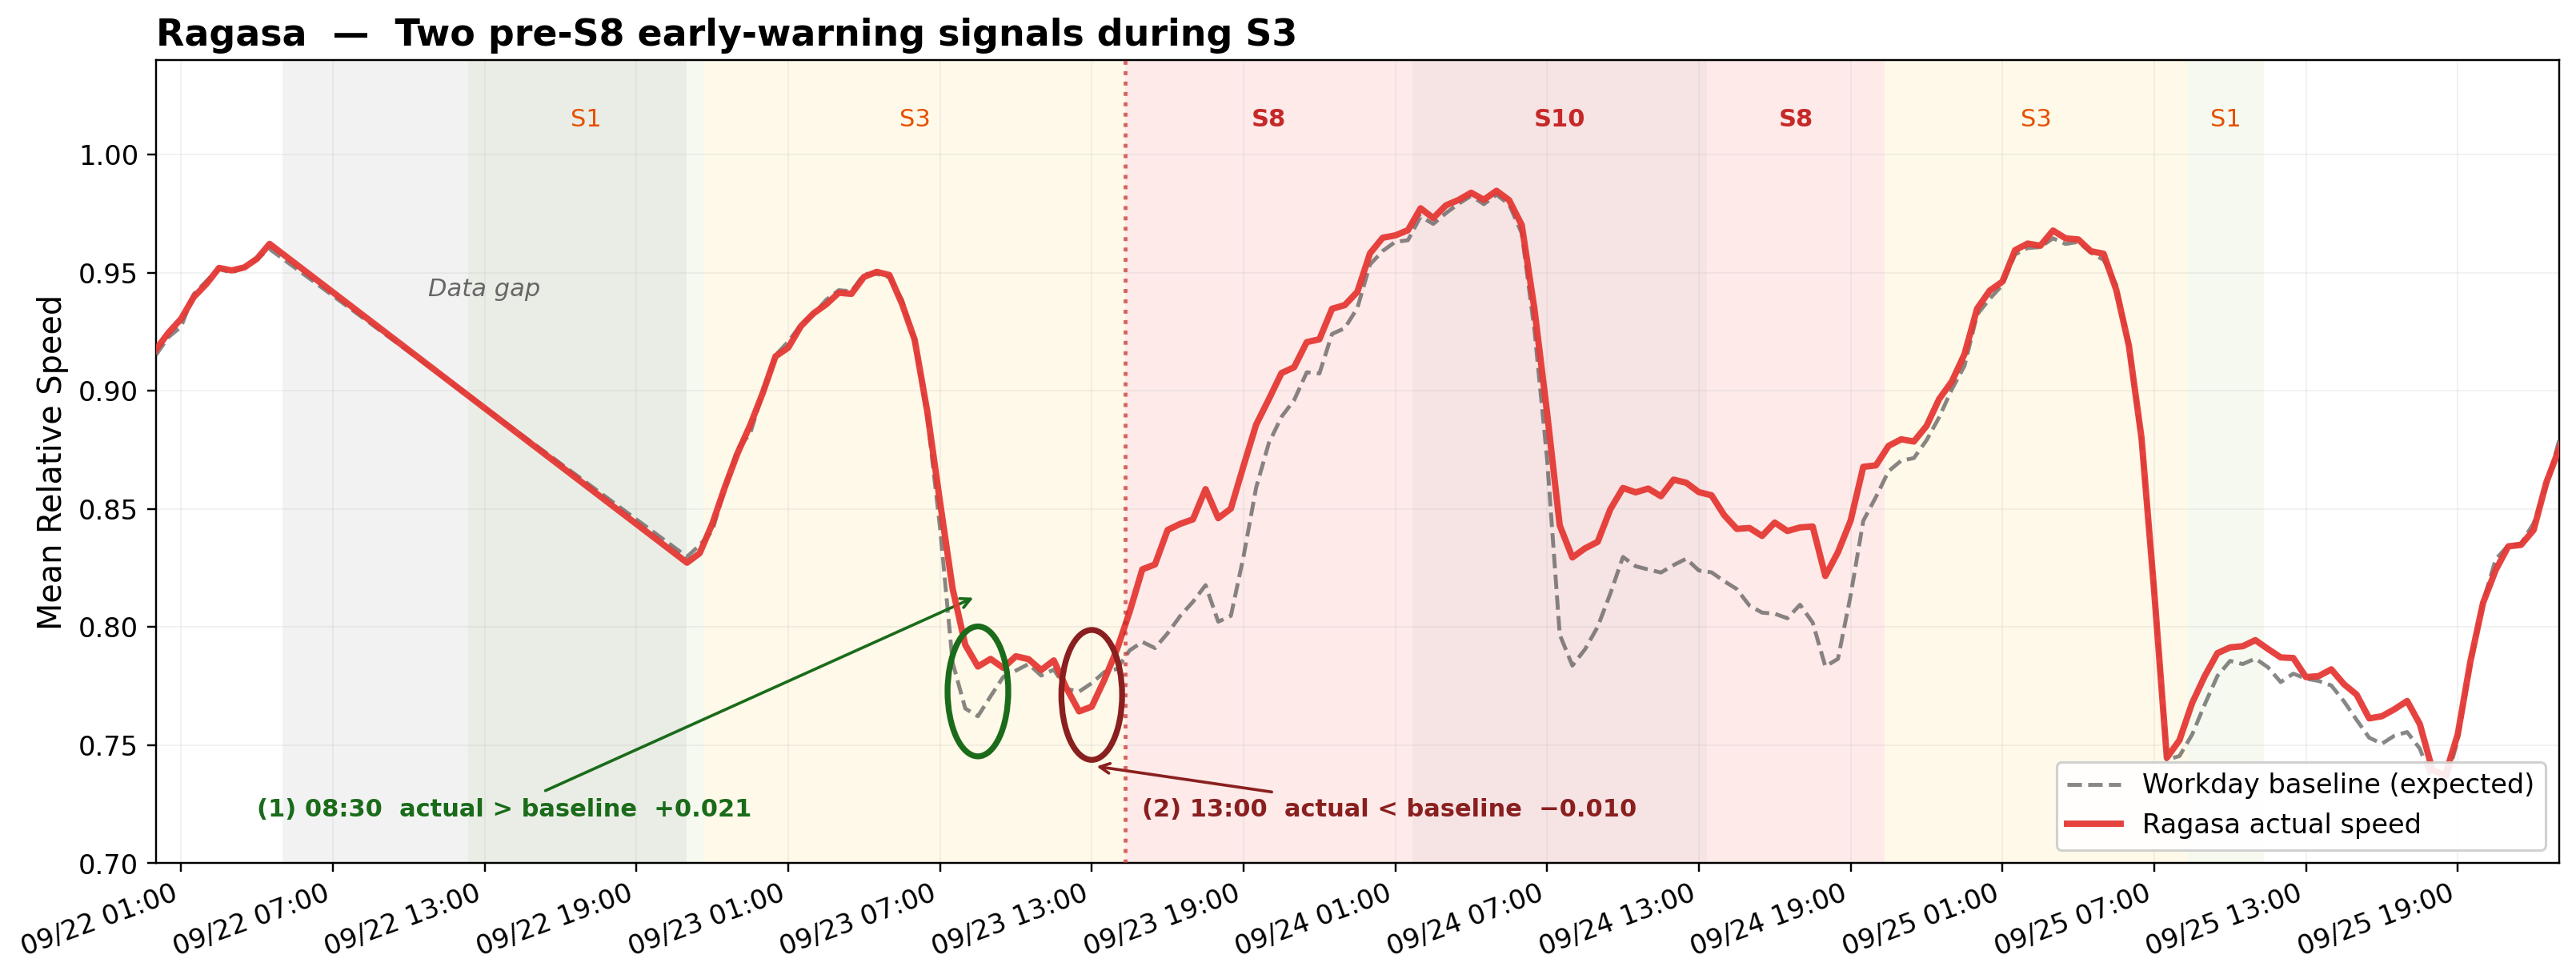
\includegraphics[width=0.95\linewidth]{图25d_Ragasa_pre_signals圈出.png}
\caption{Pre-event network speed response before Signal 8 (Ragasa). The 08:30 morning clearance (actual $>$ baseline by +0.021) and the 13:00 midday reversal (actual $<$ baseline by --0.010) are highlighted.}
\label{fig:pre_event_curve}
\end{figure}

\section{Interpretation of morning clearance}
The 08:30 pattern suggests that early warning reduced normal morning commuting pressure. Many roads that would normally be congested became faster than their baseline. This is consistent with demand suppression and anticipatory behaviour. Workers may have delayed, cancelled, or shortened trips. Employers and schools may also have adjusted schedules in response to typhoon warnings.

However, this clearance should not be interpreted as better transport performance in a simple welfare sense. Higher speed partly indicates that normal urban activity was disrupted. The road network appeared faster because demand was lower.

\section{Midday reversal}
The 13:00 pattern shows that morning clearance was not stable. Some local activity returned before Signal 8, creating slower-than-baseline roads. The midday slowdown was not a uniform network collapse. Instead, it was a polarized pattern: some roads remained faster than normal, while a larger share became slower than normal.

This pattern can be interpreted as local demand rebound. After the morning adjustment, some residents may have made school-related, shopping, or preparation trips before the stronger signal. Local incidents and road frictions may have amplified the slowdown in specific areas.

\section{Road-state transition from 08:30 to 13:00}
The transition matrix shows how road states changed between morning and midday. The diagonal cells represent roads that stayed in the same state. The off-diagonal cells represent churn. In total, 46.8\% of road-kilometres stayed in the same state, 33.1\% deteriorated, and 20.2\% improved. The most important transition was Faster to Slower, accounting for 16.52\% of matched road-kilometres.

\begin{table}[H]
\centering
\caption{Road-state transition from 08:30 to 13:00, length weighted}
\begin{tabular}{lrrrr}
\toprule
08:30 / 13:00 & F & N & S & 08:30 total \\
\midrule
F & 14.88\% & 11.02\% & 16.52\% & 42.42\% \\
N & 8.44\% & 21.37\% & 5.52\% & 35.33\% \\
S & 8.26\% & 3.46\% & 10.53\% & 22.24\% \\
\midrule
13:00 total & 31.57\% & 35.85\% & 32.58\% & 100\% \\
\bottomrule
\end{tabular}
\end{table}

This result shows that the pre-event period was dynamic. Morning traffic clearance was only temporary. The network shifted from early relief to midday churn, and the main change was the reversal of roads from faster-than-baseline to slower-than-baseline.

\begin{figure}[H]
\centering
\begin{subfigure}[t]{0.32\linewidth}
  \centering
  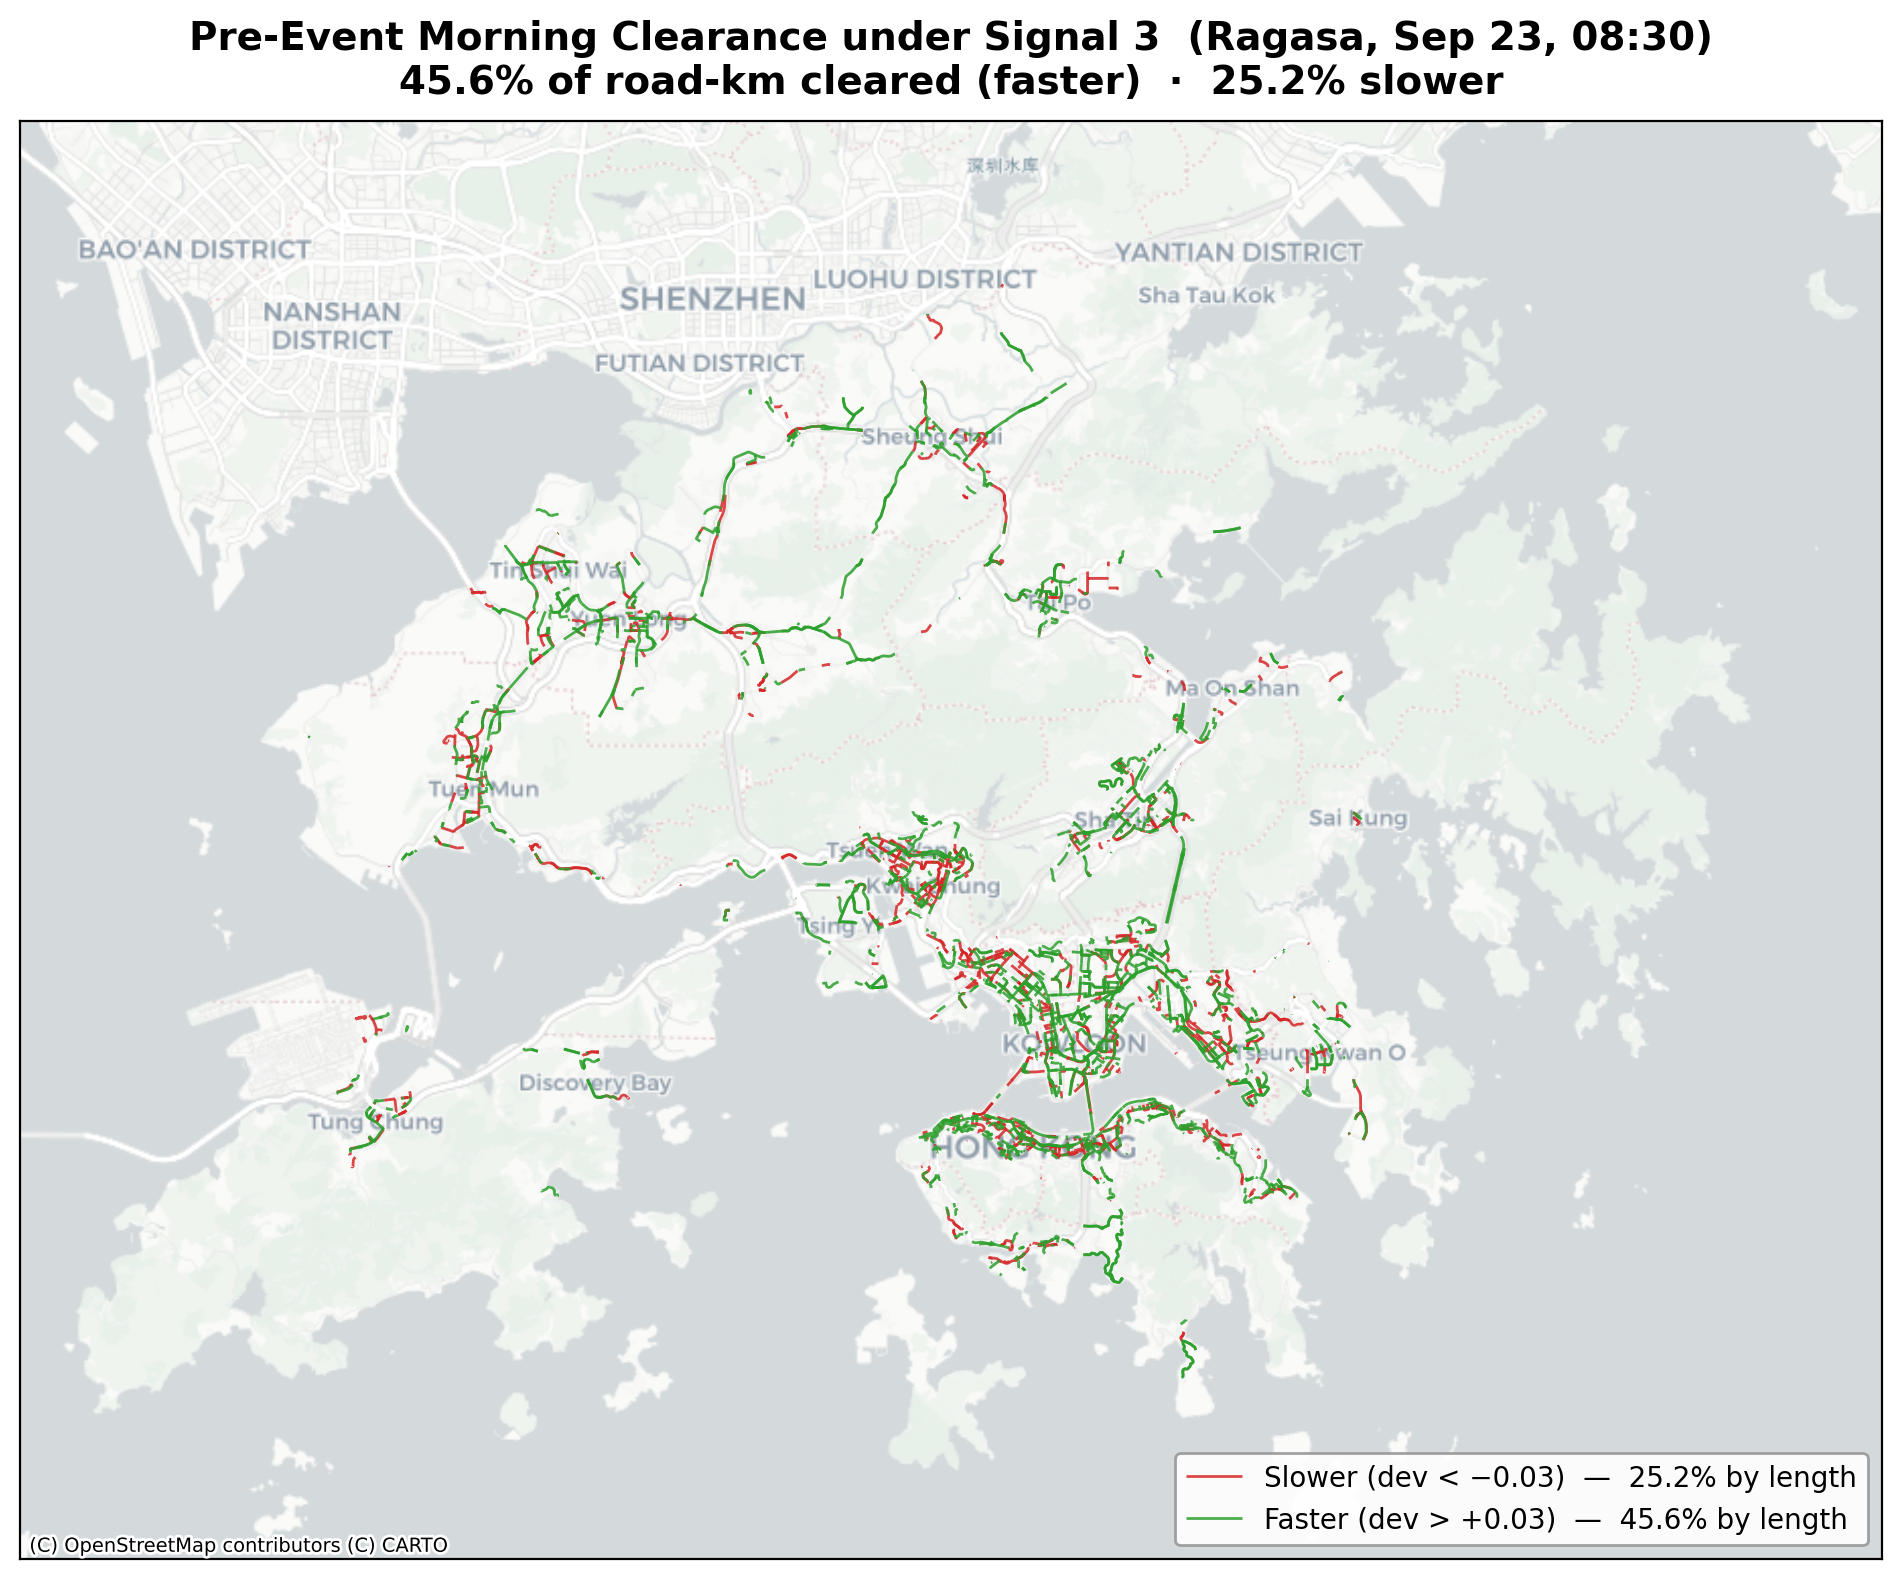
\includegraphics[width=\linewidth]{图50d_pre_event_morning_clearance.png}
  \caption{08:30 morning clearance}
\end{subfigure}\hfill
\begin{subfigure}[t]{0.32\linewidth}
  \centering
  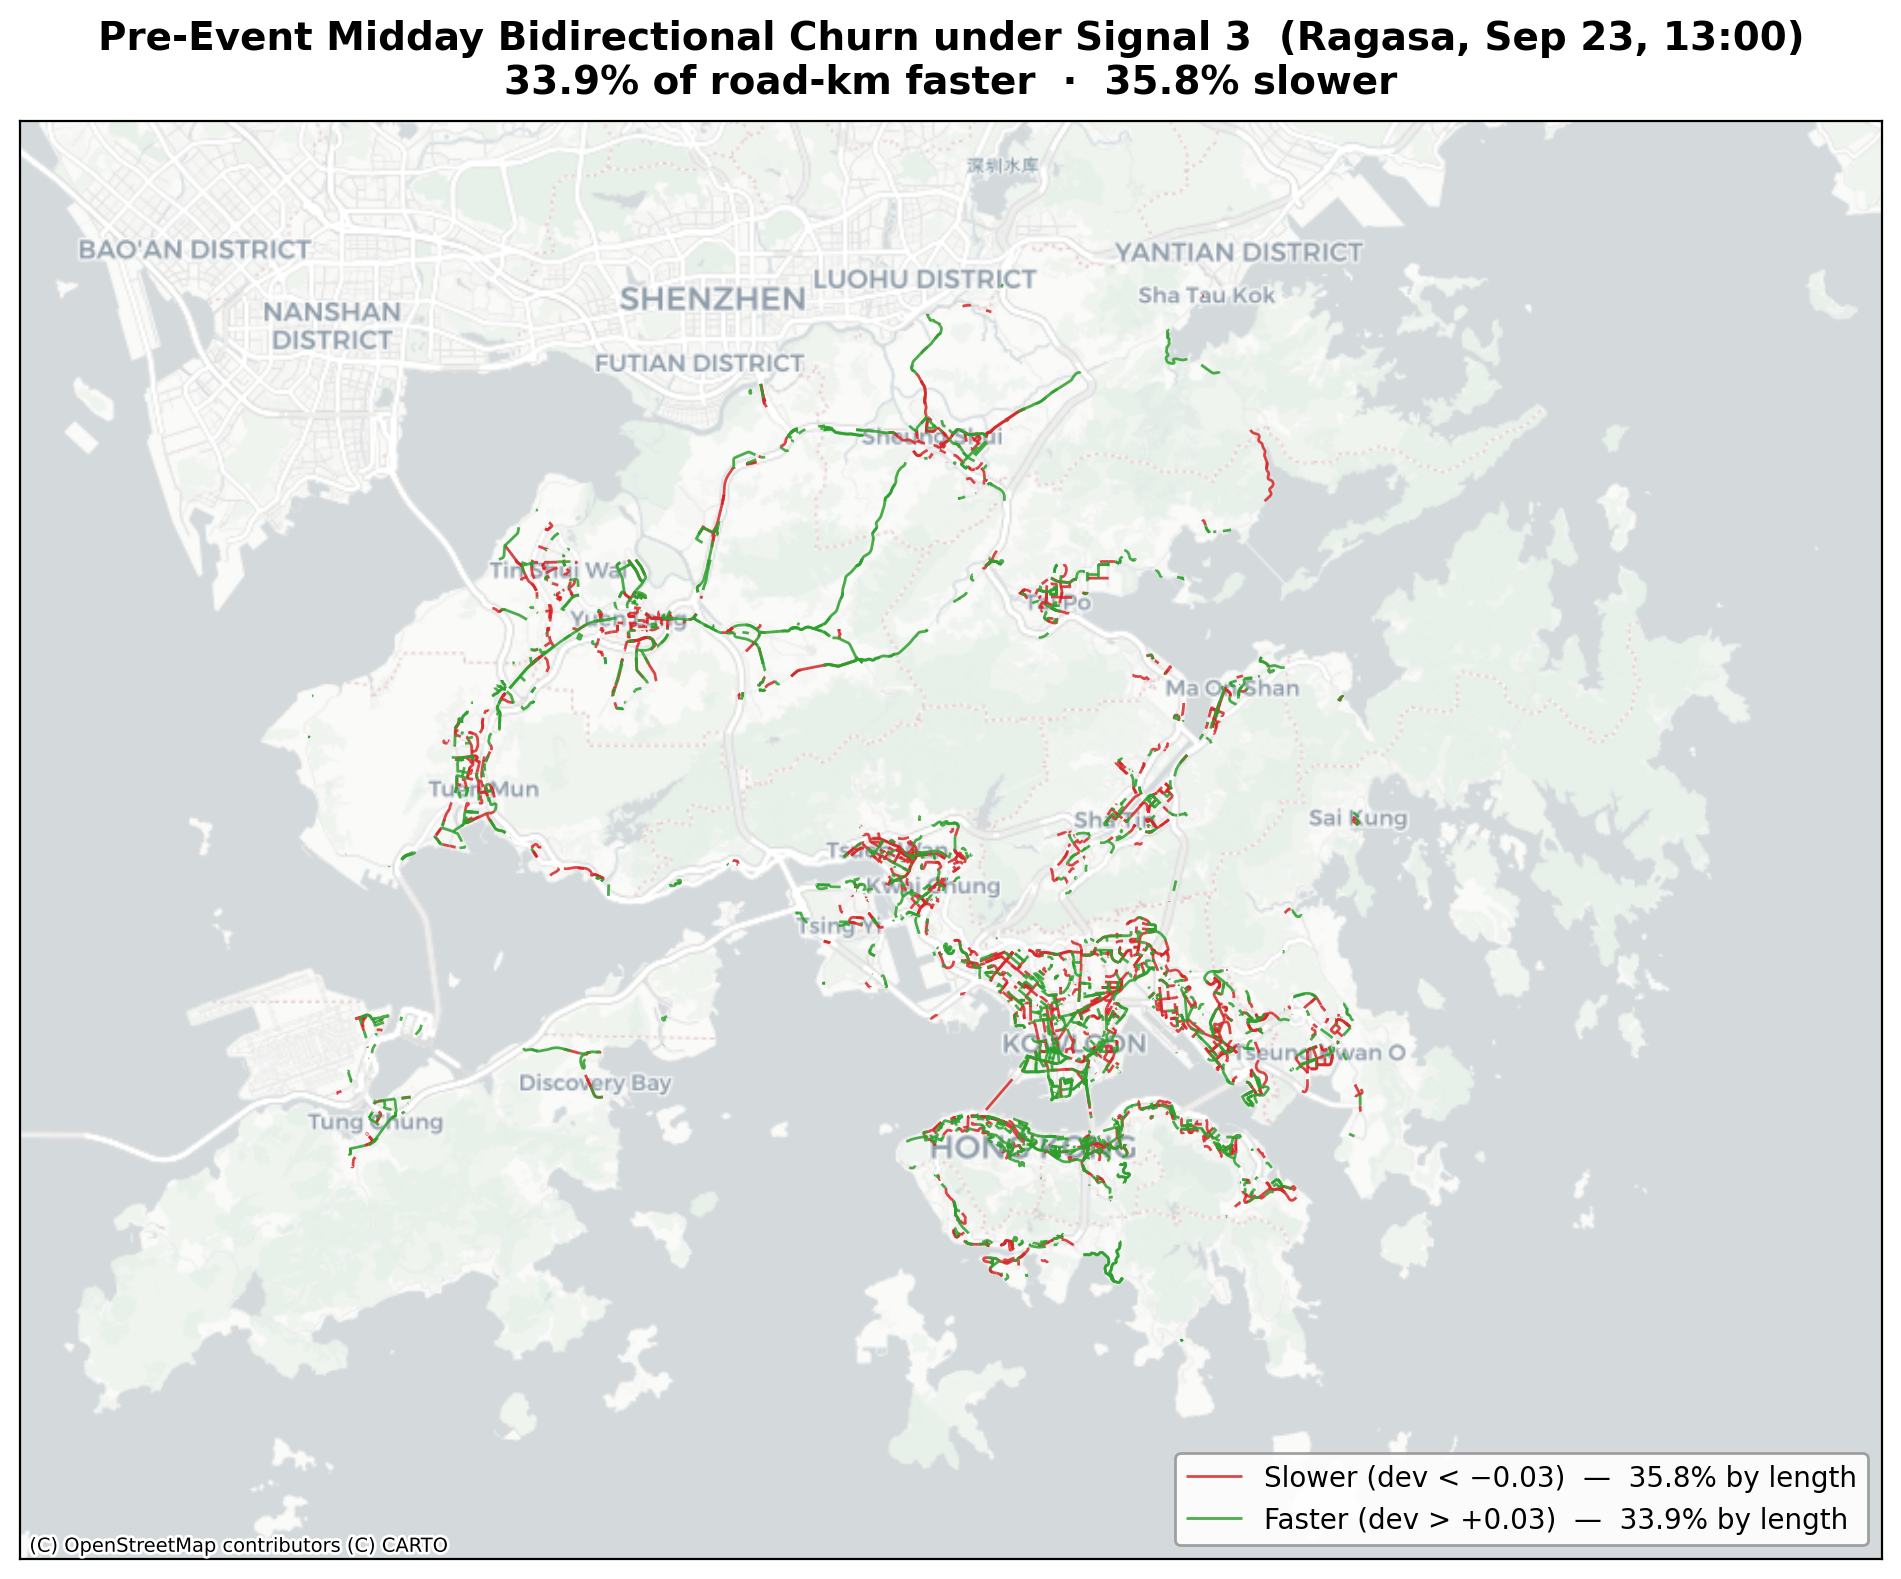
\includegraphics[width=\linewidth]{图50e_pre_event_midday_churn.png}
  \caption{13:00 midday reversal}
\end{subfigure}\hfill
\begin{subfigure}[t]{0.32\linewidth}
  \centering
  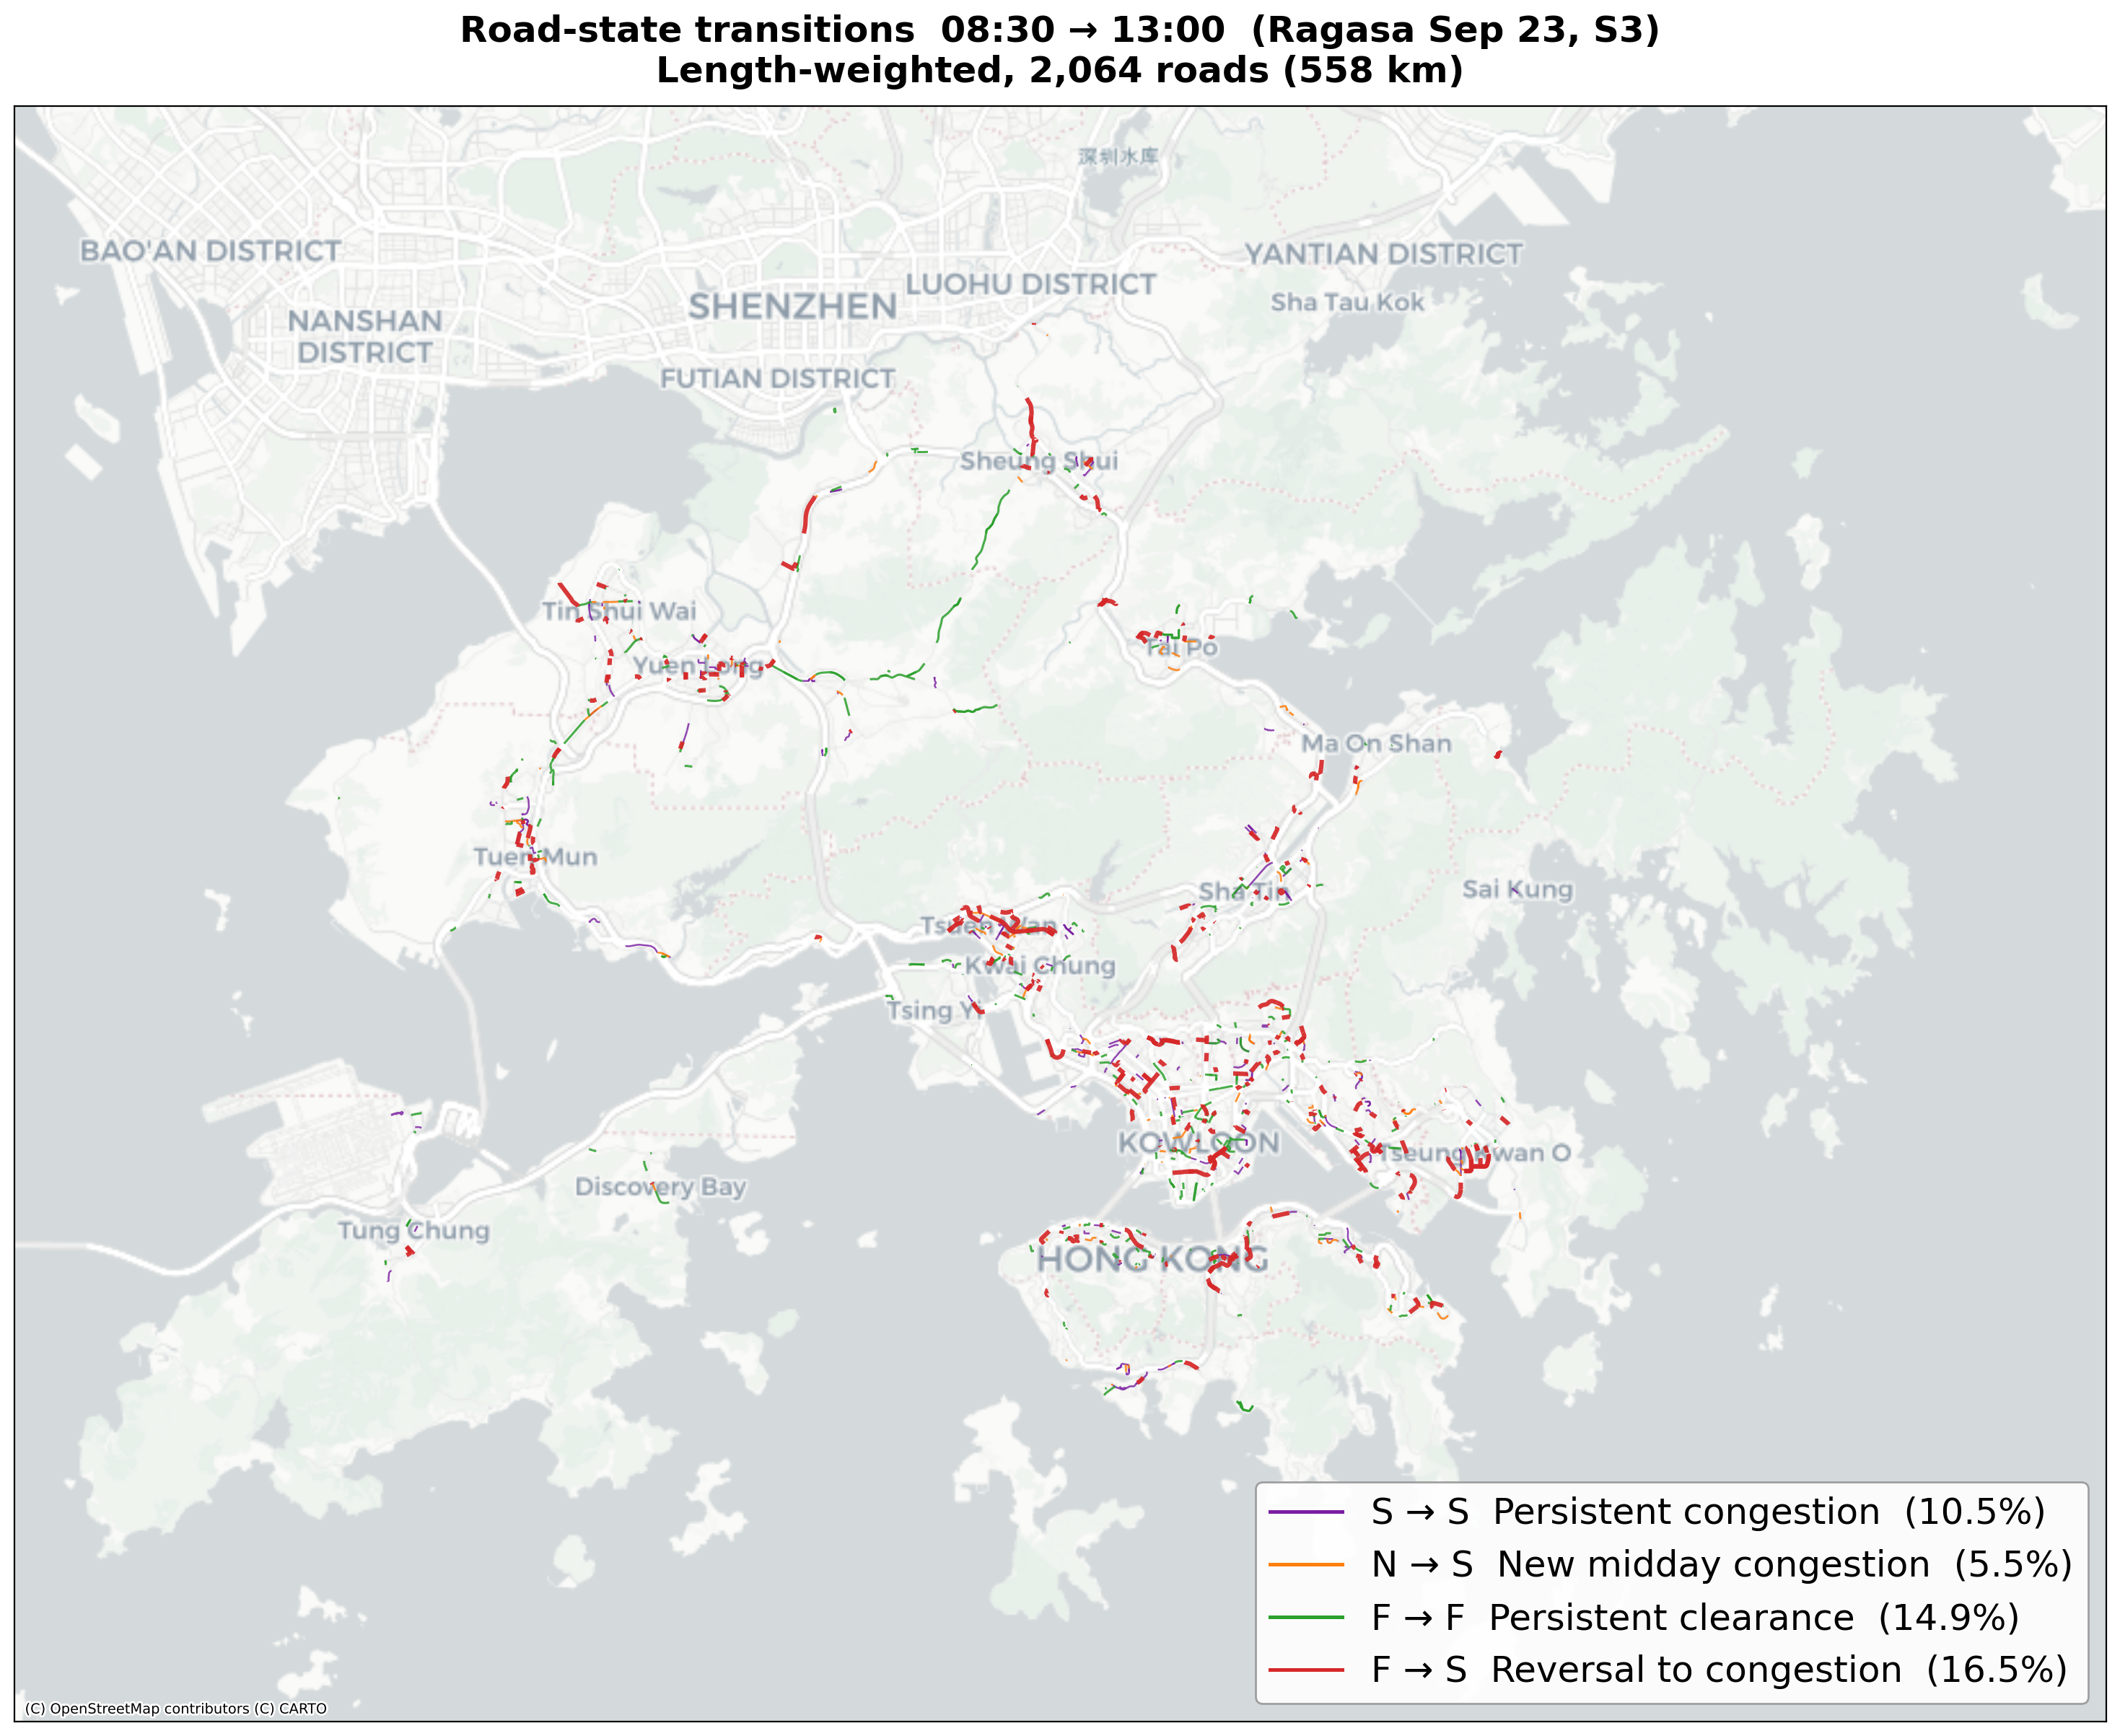
\includegraphics[width=\linewidth]{图50g_transition_map.png}
  \caption{08:30 $\rightarrow$ 13:00 road-state transitions}
\end{subfigure}
\caption{Spatial distribution of morning clearance, midday reversal, and road-state transitions (Ragasa, Sep 23, Signal 3).}
\label{fig:pre_event_maps}
\end{figure}

\section{Regression evidence for morning clearance}
The morning clearance model examines which roads were more likely to become faster than baseline at 08:30. The dependent variable equals 1 if the road deviation is greater than +0.03. The model includes 1,465 roads with complete demographic and built-environment data. About 47.5\% of roads are classified as cleared. The best specification has an AUC of 0.621.

\begin{table}[H]
\centering
\caption{Summary of morning clearance regression evidence}
\begin{tabularx}{\textwidth}{lclX}
\toprule
Predictor & Direction & Odds ratio & Interpretation \\
\midrule
Employee-resident ratio & Positive & 2.60--2.88*** & Roads in areas with stronger employment-residential imbalance were more likely to clear. \\
Working-population ratio & Negative & 0.33--0.36* & Areas with higher working-population concentration were harder to clear in the current specification. \\
School count within 1 km & Positive & 1.30** & Roads near more schools were more likely to clear. \\
Distance to coast & Positive & about 1.18* & Inland roads were more likely to clear than coastal roads. \\
\bottomrule
\end{tabularx}
\end{table}

The pattern supports demand suppression and anticipatory behaviour rather than uniform physical disruption. Roads that normally experience commuting pressure appear to have gained relief when usual travel was reduced.

\section{Regression evidence for midday slowdown}
The midday model examines which roads became slower than baseline at 13:00. The dependent variable equals 1 if the road deviation is less than -0.03. The model includes 1,721 roads in the current specification. About 41.3\% of roads are classified as slowed. The model has an AUC of 0.637 and McFadden $R^2$ of 0.0479.

\begin{table}[H]
\centering
\caption{Summary of midday slowdown regression evidence}
\begin{tabularx}{\textwidth}{lclX}
\toprule
Predictor & Direction & Odds ratio & Interpretation \\
\midrule
School count within 1 km & Positive & 1.46*** & Roads near schools were more likely to slow down. \\
Retail density & Positive & 1.51* & Retail streets were more vulnerable to midday slowdown. \\
Incident count within 500 m & Positive & 1.16* & Nearby incidents increased the likelihood of slowdown. \\
Tourism density & Negative & 0.46*** & Tourism-dense areas were less likely to slow down in this period. \\
\bottomrule
\end{tabularx}
\end{table}

The result suggests that the midday reversal was concentrated around schools, retail streets, incident-prone roads, and selected residential areas. It was not a typhoon-wide speed loss, but a localized rebound and friction pattern.

% =========================
% Chapter 6 During
% =========================
\chapter{During-Event Results: Demand Suppression and Localized Disruption}

\section{Overall during-event pattern}
During high-warning typhoon periods, average network speed was often higher than the matched baseline. This does not mean that typhoons improved road performance. Instead, the most plausible explanation is that travel demand was strongly suppressed. When many people stayed home, roads moved closer to free-flow conditions.

The presentation results show that the overall during-event mean deviation was positive. The mean deviation reached about +0.033 in one during-event summary, with 15.1\% of roads faster, 1.8\% slower, and 83.1\% near normal. The relief was not evenly distributed. Normally congested roads benefited the most.

\section{Relief concentrated on normally congested roads}
Roads are grouped by baseline congestion level. The most congested baseline group experienced the strongest positive deviation during the event. In the first quintile, the mean speed deviation reached +0.096, with 44\% faster roads. In the second quintile, the mean deviation was +0.061, with 23\% faster roads. In contrast, the least congested roads showed almost no improvement.

\begin{table}[H]
\centering
\caption{During-event deviation by baseline congestion group}
\begin{tabular}{lrr}
\toprule
Baseline congestion group & Mean deviation & Share faster \\
\midrule
Q1, most congested & +0.096 & 44\% \\
Q2 & +0.061 & 23\% \\
Q3 & +0.009 & 9\% \\
Q4 & -0.001 & 5\% \\
Q5, least congested & -0.002 & 5\% \\
\bottomrule
\end{tabular}
\end{table}

This pattern is important because it shows that during-event relief was conditional on normal congestion. The roads that had the most room to improve under reduced demand gained the most speed. Roads already close to free-flow speed had little room for further improvement.

\begin{figure}[H]
\centering
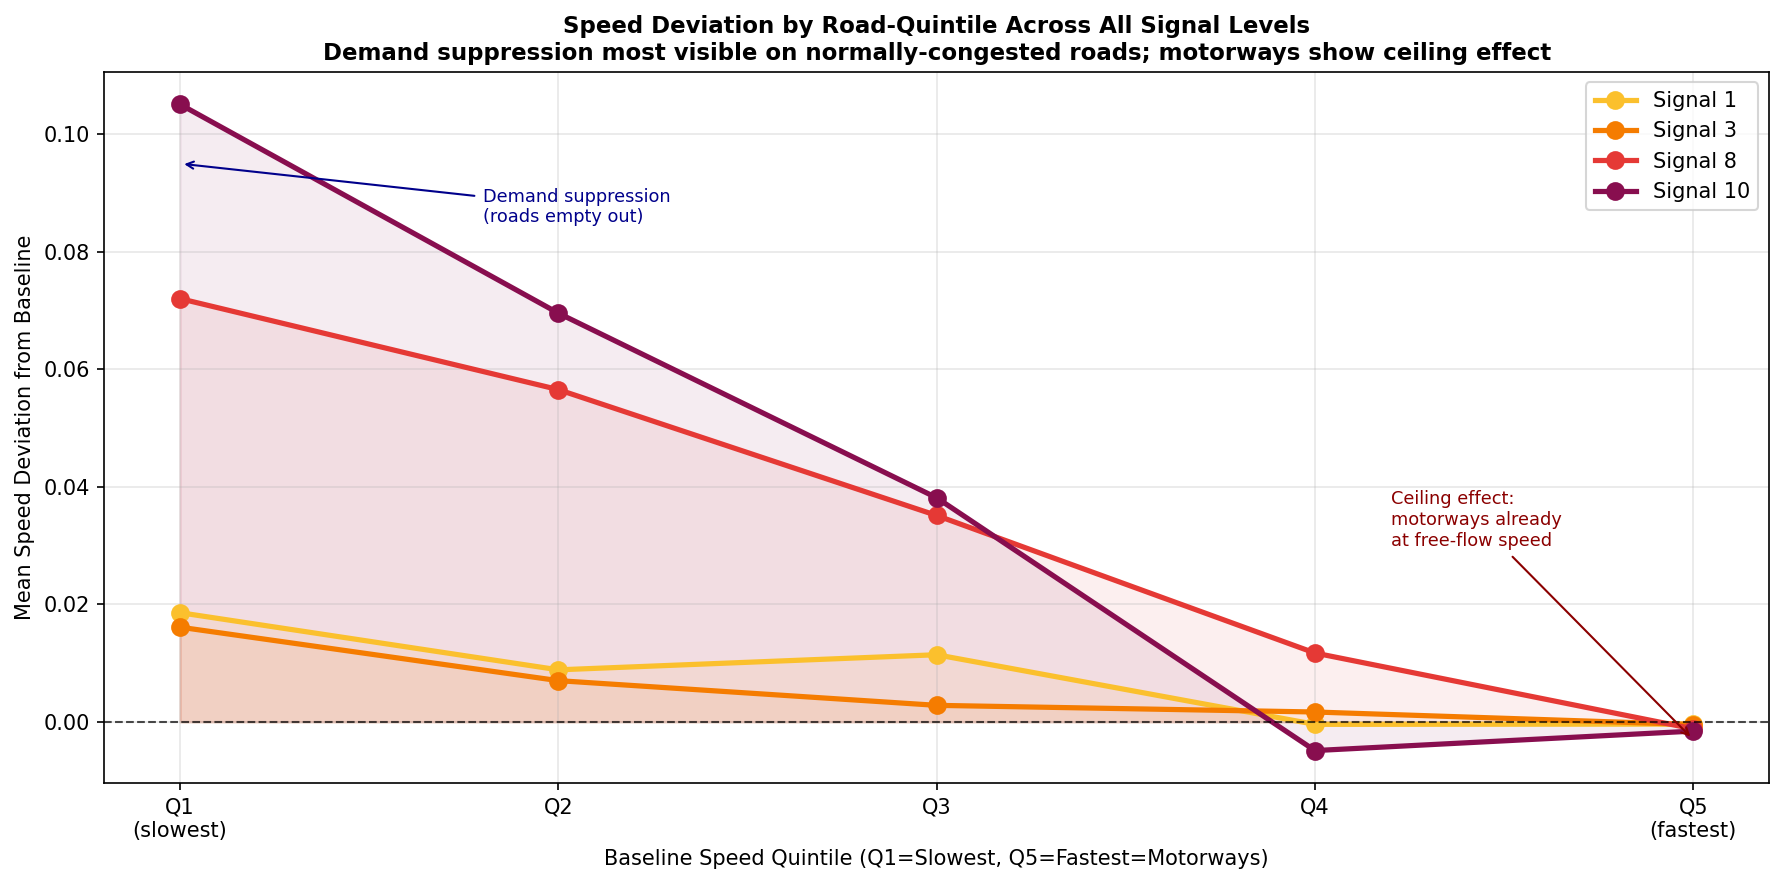
\includegraphics[width=0.9\linewidth]{图13_五分位偏差信号等级梯度.png}
\caption{Mean speed deviation from baseline by road-quintile across all signal levels. Demand suppression is most visible on normally congested roads (Q1), while motorway-class roads (Q5) show a ceiling effect.}
\label{fig:during_quintile}
\end{figure}

\section{Commercial density and baseline congestion}
A second descriptive grouping shows that roads in higher commercial-density quintiles had larger raw speed gains. However, after controlling for baseline speed, commercial POI density was not significant in the regression insight reported in the presentation. This suggests that commercial-area gains are mostly explained by normal congestion: commercial centres are usually congested, so they benefit more when demand is suppressed.

\section{Morning peak under demand suppression}
During the event, the morning peak did not disappear completely. The curve shifted upward, but retained a similar U-shape. The baseline 06:00 speed was 0.835 and dropped to 0.716 at the trough, a drop of -0.119. Under Signal 3, the 06:00 speed was 0.922 and the trough was 0.782, a drop of -0.140. Under Signal 10, the 06:00 speed was 0.970 and the trough was 0.829, a drop of -0.141.

\begin{table}[H]
\centering
\caption{Morning peak persistence under demand suppression}
\begin{tabular}{lrrr}
\toprule
Group & 06:00 speed & Trough speed & Drop \\
\midrule
Baseline & 0.835 & 0.716 & -0.119 \\
Signal 3 & 0.922 & 0.782 & -0.140 \\
Signal 10 & 0.970 & 0.829 & -0.141 \\
\bottomrule
\end{tabular}
\end{table}

\begin{figure}[H]
\centering
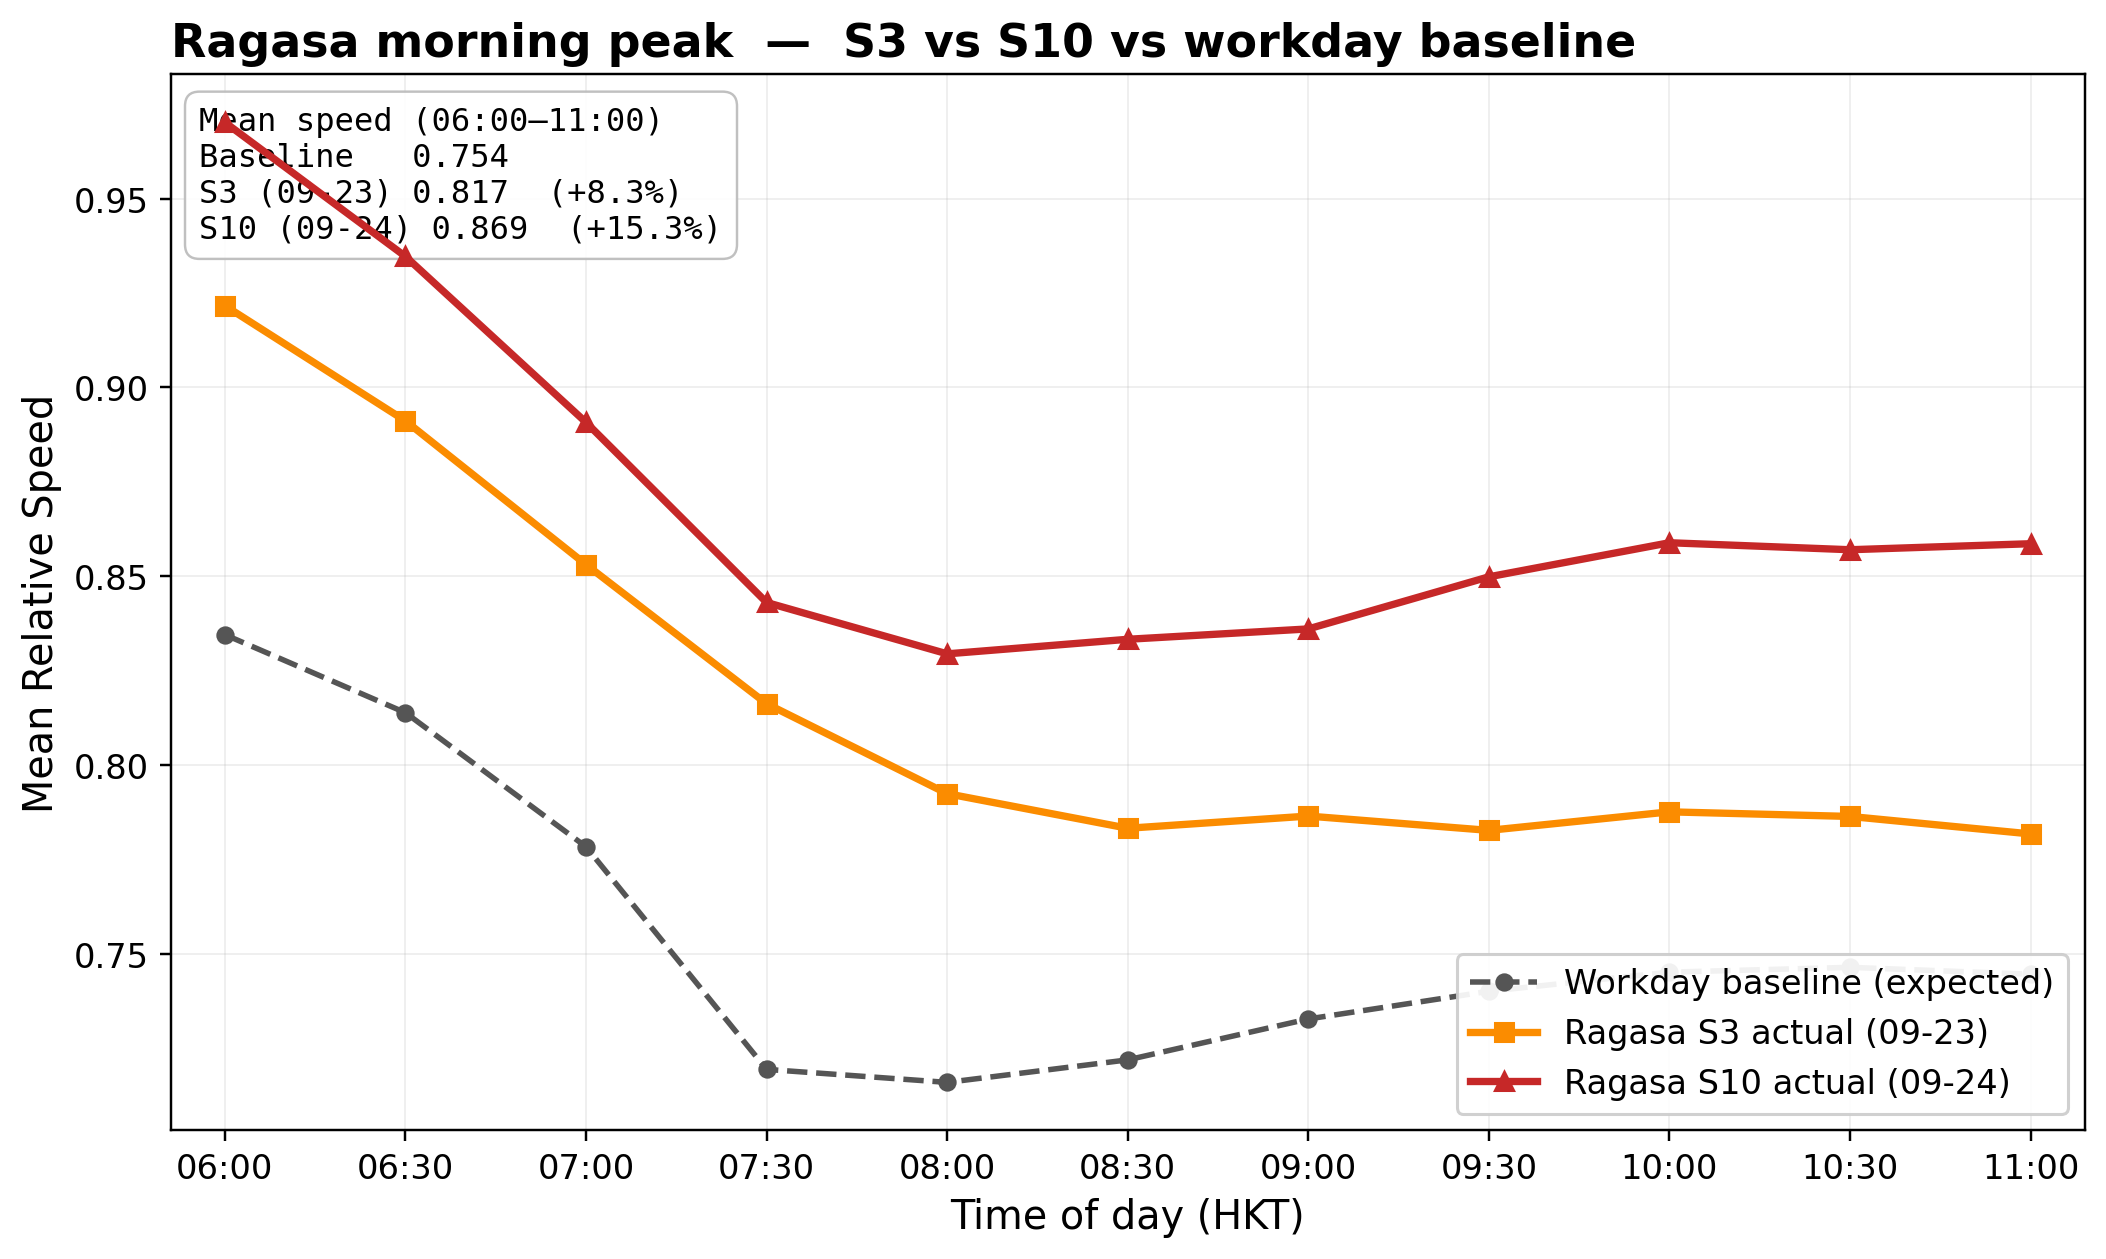
\includegraphics[width=0.85\linewidth]{图25e_Ragasa_morning_S3_S10_baseline.png}
\caption{Ragasa morning peak (06:00--11:00) under Signal 3 and Signal 10 compared with the matched workday baseline. The curve shifts upward but retains a similar U-shape.}
\label{fig:morning_peak}
\end{figure}

This means that demand suppression raised the overall level of the curve, but it did not fully flatten temporal traffic structure. Some morning travel rhythm remained.

\section{Evening peak and partial demand reactivation}
The evening trough was much shallower than normal. For the baseline, the 18:00 speed was 0.707. Under rising Signal 8, the 18:00 speed was 0.846 and the trough was 0.841. Under falling Signal 8, the 18:00 speed was 0.822 and the trough was also 0.822. Falling Signal 8 had more observed roads and lower speed than rising Signal 8, suggesting partial demand reactivation after Signal 10.

\begin{table}[H]
\centering
\caption{Evening peak comparison under rising and falling Signal 8}
\begin{tabular}{lrrr}
\toprule
Group & 18:00 speed & Trough speed & Drop \\
\midrule
Baseline & 0.707 & 0.707 & -0.039 \\
Rising Signal 8 & 0.846 & 0.841 & -0.081 \\
Falling Signal 8 & 0.822 & 0.822 & -0.063 \\
\bottomrule
\end{tabular}
\end{table}

\begin{figure}[H]
\centering
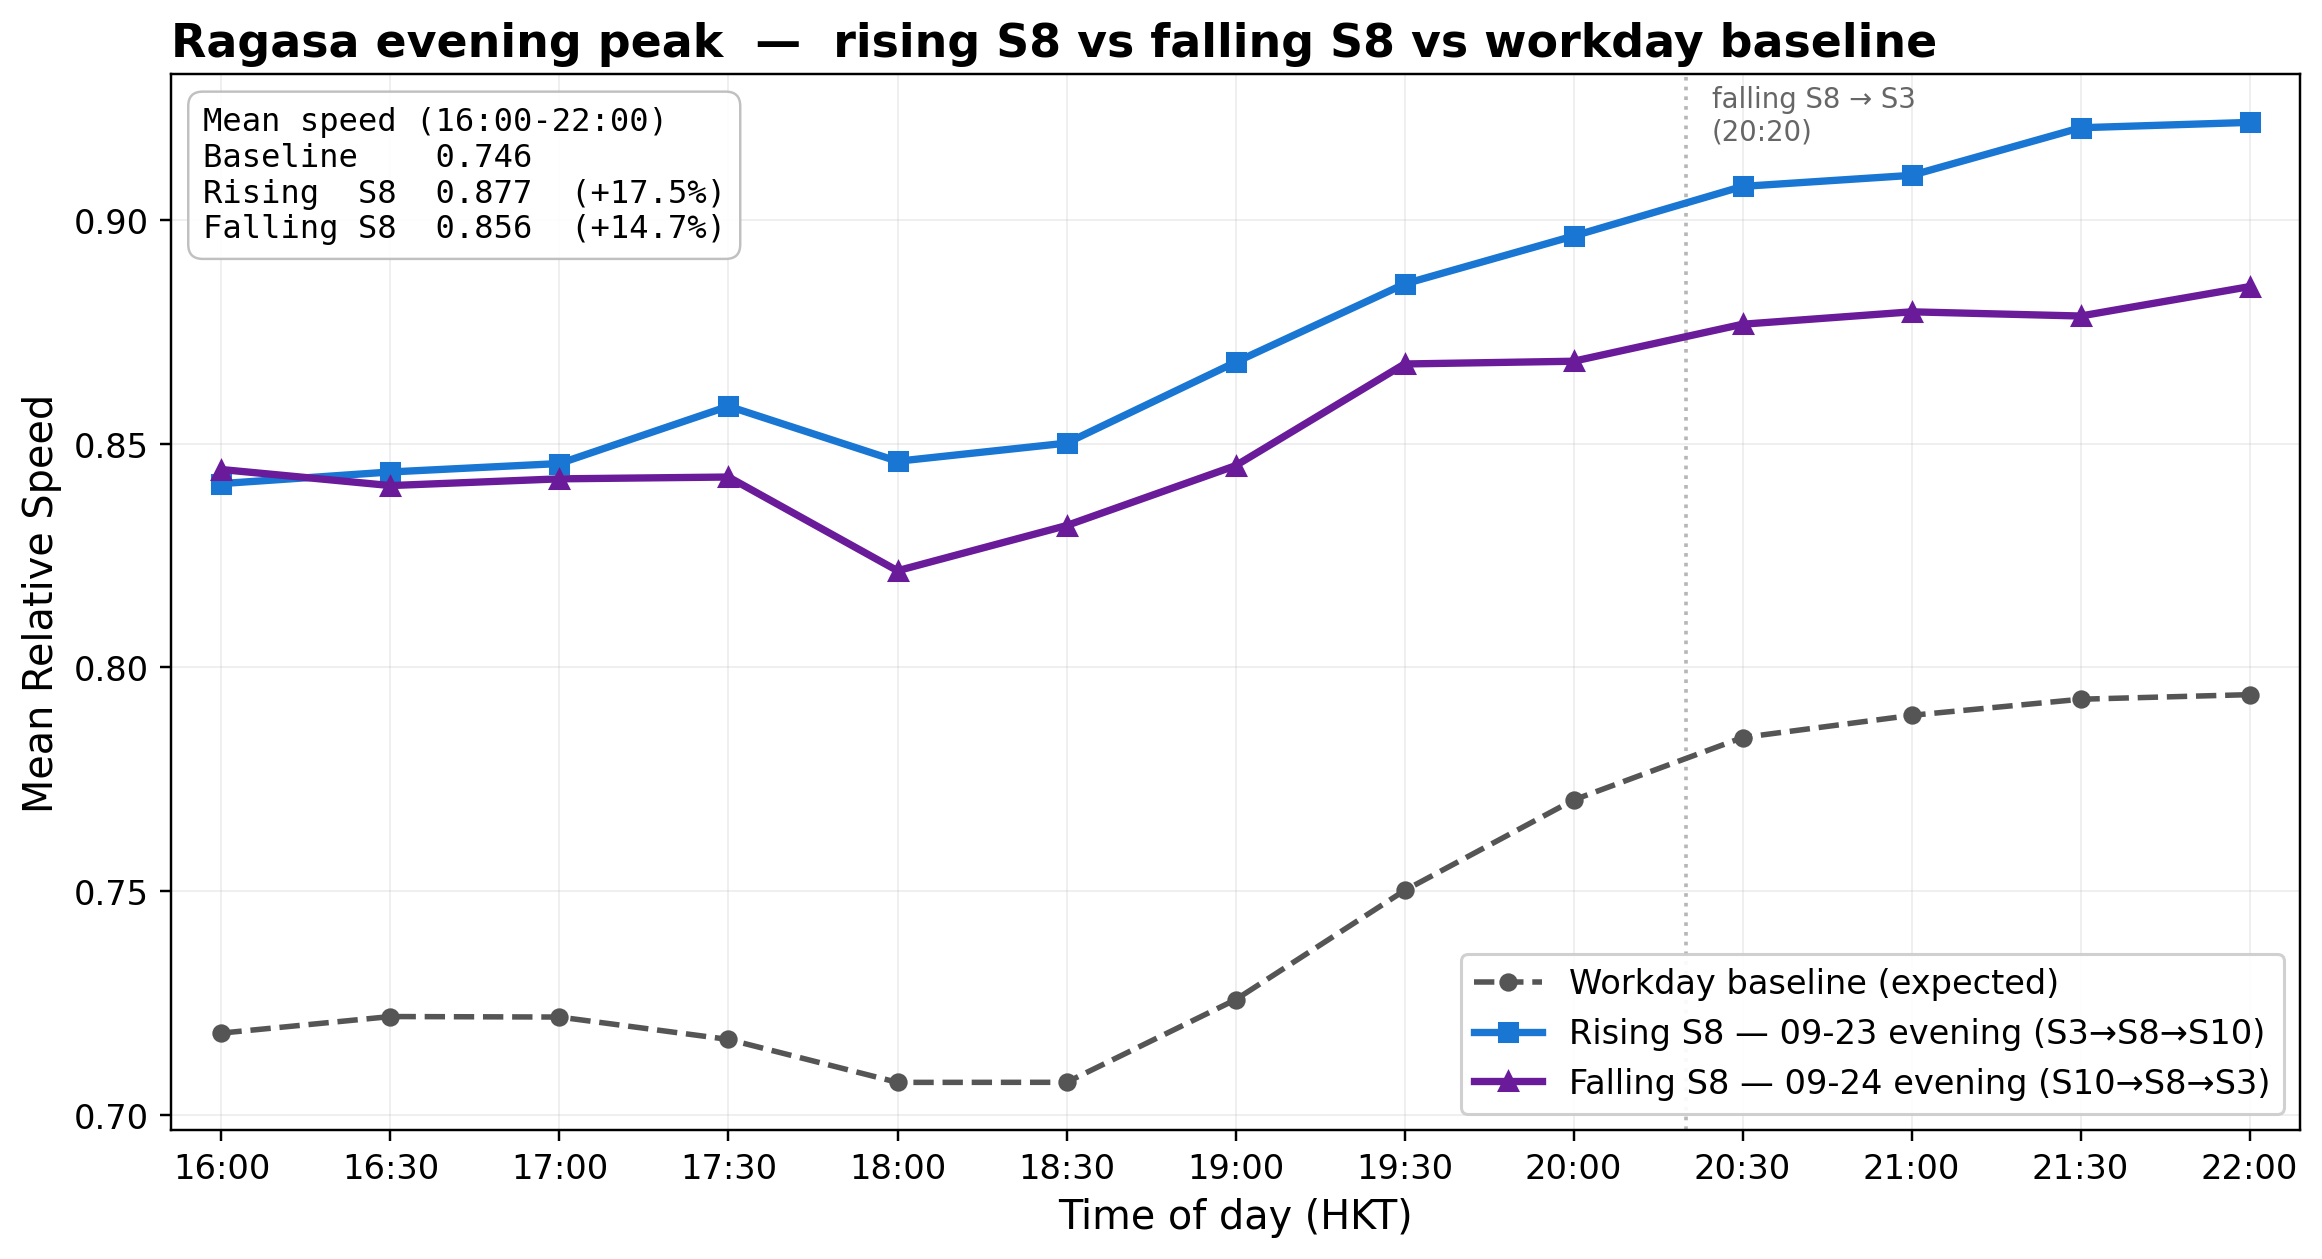
\includegraphics[width=0.85\linewidth]{图25f_Ragasa_evening_S8_compare.png}
\caption{Ragasa evening peak (16:00--22:00): rising Signal 8 (S3$\rightarrow$S10) and falling Signal 8 (S10$\rightarrow$S3) compared with the matched workday baseline.}
\label{fig:evening_peak}
\end{figure}

\section{Heterogeneity across rising, peak, and falling windows}
To probe whether during-event speed change is uniform across the signal sequence, the Ragasa event is split into three windows: rising Signal 8 (S3$\rightarrow$S10 on 09-23), peak Signal 10+S8 (09-24), and falling Signal 8 (S10$\rightarrow$S3 on 09-25). Within each window, roads are grouped into baseline-congestion quintiles (Q1 slowest to Q5 free-flow) and into commercial-density quintiles (low to high POI count within 500 m).

\begin{figure}[H]
\centering
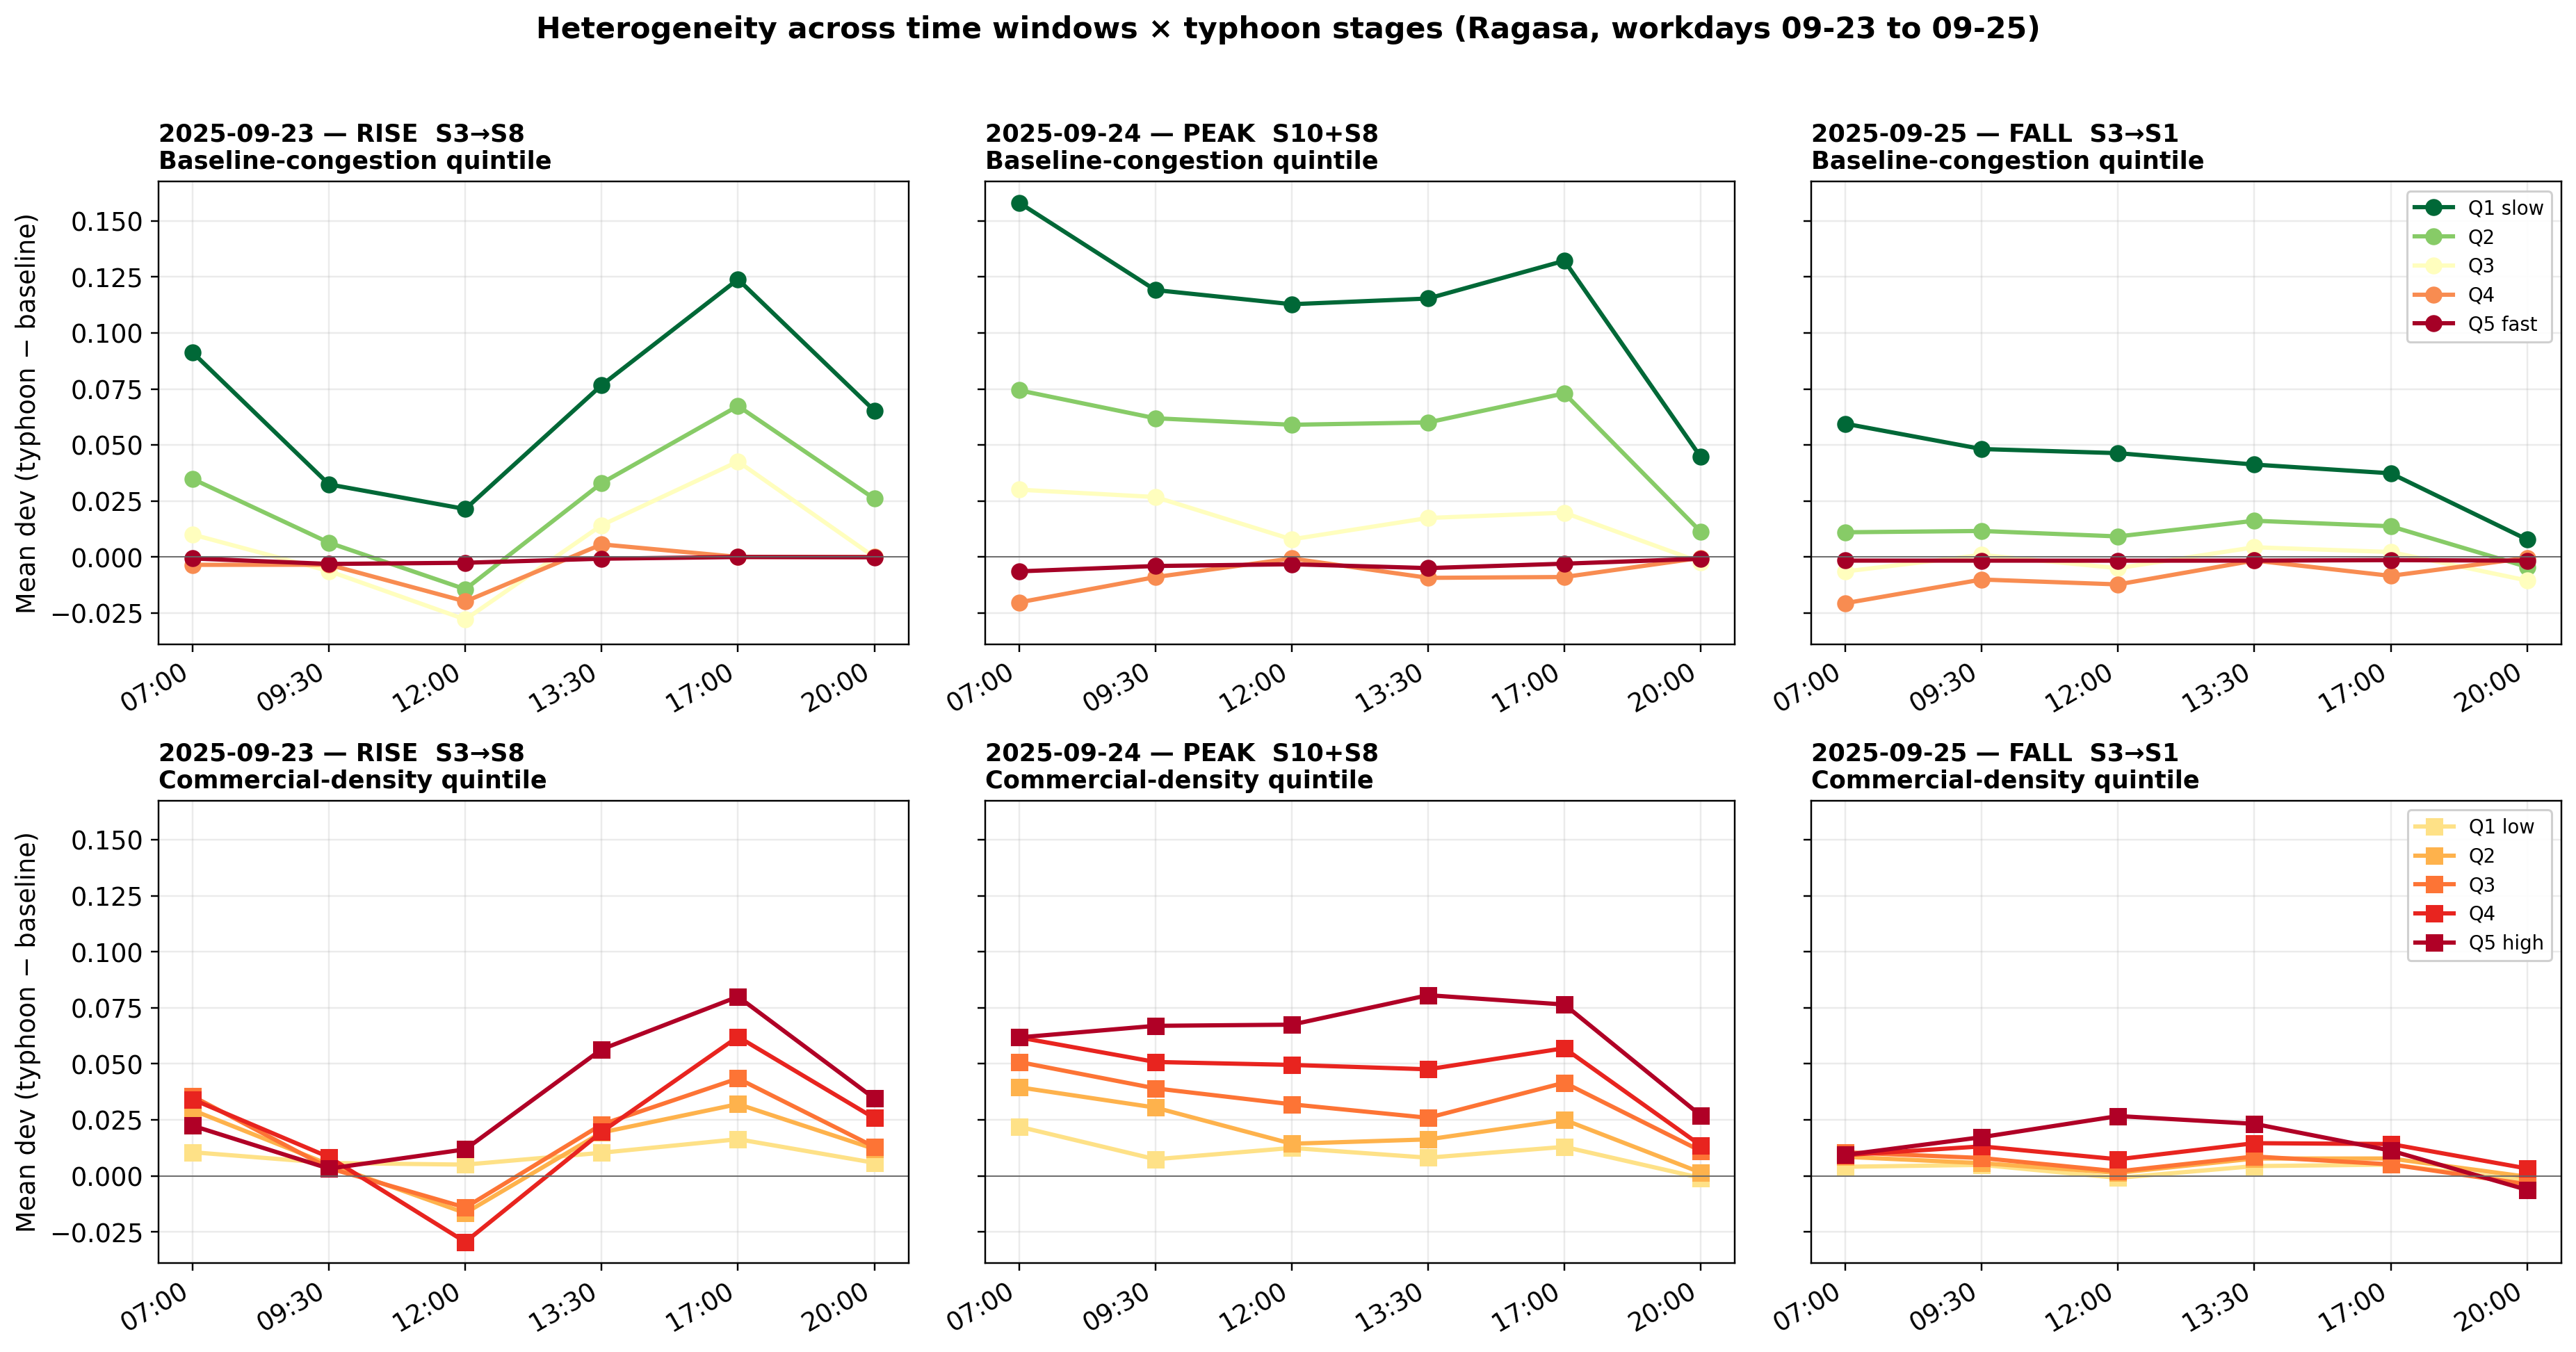
\includegraphics[width=0.95\linewidth]{图25h_heterogeneity_panel.png}
\caption{Heterogeneity across time windows and typhoon stages (Ragasa, 09-23 to 09-25). Top row groups roads by baseline-congestion quintile; bottom row by commercial-density quintile.}
\label{fig:heterogeneity_panel}
\end{figure}

Three patterns emerge. First, baseline congestion is by far the strongest moderator: Q1 roads experience deviations above +0.10 on the peak day, while Q5 roads stay near zero across all three windows. This is the ``ceiling effect''---roads already close to free-flow speed have no room to gain. Second, the peak window (09-24) is when commercial-density gradients become most visible: high-commercial quintiles show stronger positive deviation than low-commercial ones, consistent with demand suppression in activity centres. Third, on the falling day (09-25 morning) the pattern weakens markedly even though Signal 8 was still in effect during part of the window; this suggests demand reactivation begins before official downgrade.

Table \ref{tab:het_by_window} summarises mean deviation in Q1 of the baseline-congestion grouping across selected time windows for the three days.

\begin{table}[H]
\centering
\caption{Mean speed deviation for Q1 baseline-congestion roads across time windows (Ragasa)}
\label{tab:het_by_window}
\begin{tabular}{lrrr}
\toprule
Time window & 09-23 (rising S8) & 09-24 (peak S10+S8) & 09-25 (falling S3) \\
\midrule
Morning peak (07--10) & +0.091 & +0.158 & +0.059 \\
Mid-morning (10--12)  & +0.032 & +0.119 & +0.048 \\
Lunch (12--14)        & +0.021 & +0.113 & +0.046 \\
Afternoon (14--17)    & +0.077 & +0.115 & +0.041 \\
Evening peak (17--19) & +0.124 & +0.132 & +0.037 \\
Late evening (19--22) & +0.065 & +0.045 & +0.008 \\
\bottomrule
\end{tabular}
\end{table}

The peak day shows the highest and most temporally stable relief, while the rising and falling days exhibit characteristic intra-day swings: the rising day has a deep midday dip (the same midday reversal documented in Chapter 5), and the falling day shows monotonic decay toward zero as demand returns.

\section{Observation disappearance during high signals}
A key concern with floating-car data during typhoons is that elevated mean speed could partly reflect survivorship: low-speed roads stop being observed because their probe vehicle counts fall below TomTom's minimum threshold. To test this, all 165,998 roads with at least one baseline observation are classified by the latest signal level at which they still produce data: never observed, lost at S3, lost at S8, lost at S10, or survived through S10.

\begin{figure}[H]
\centering
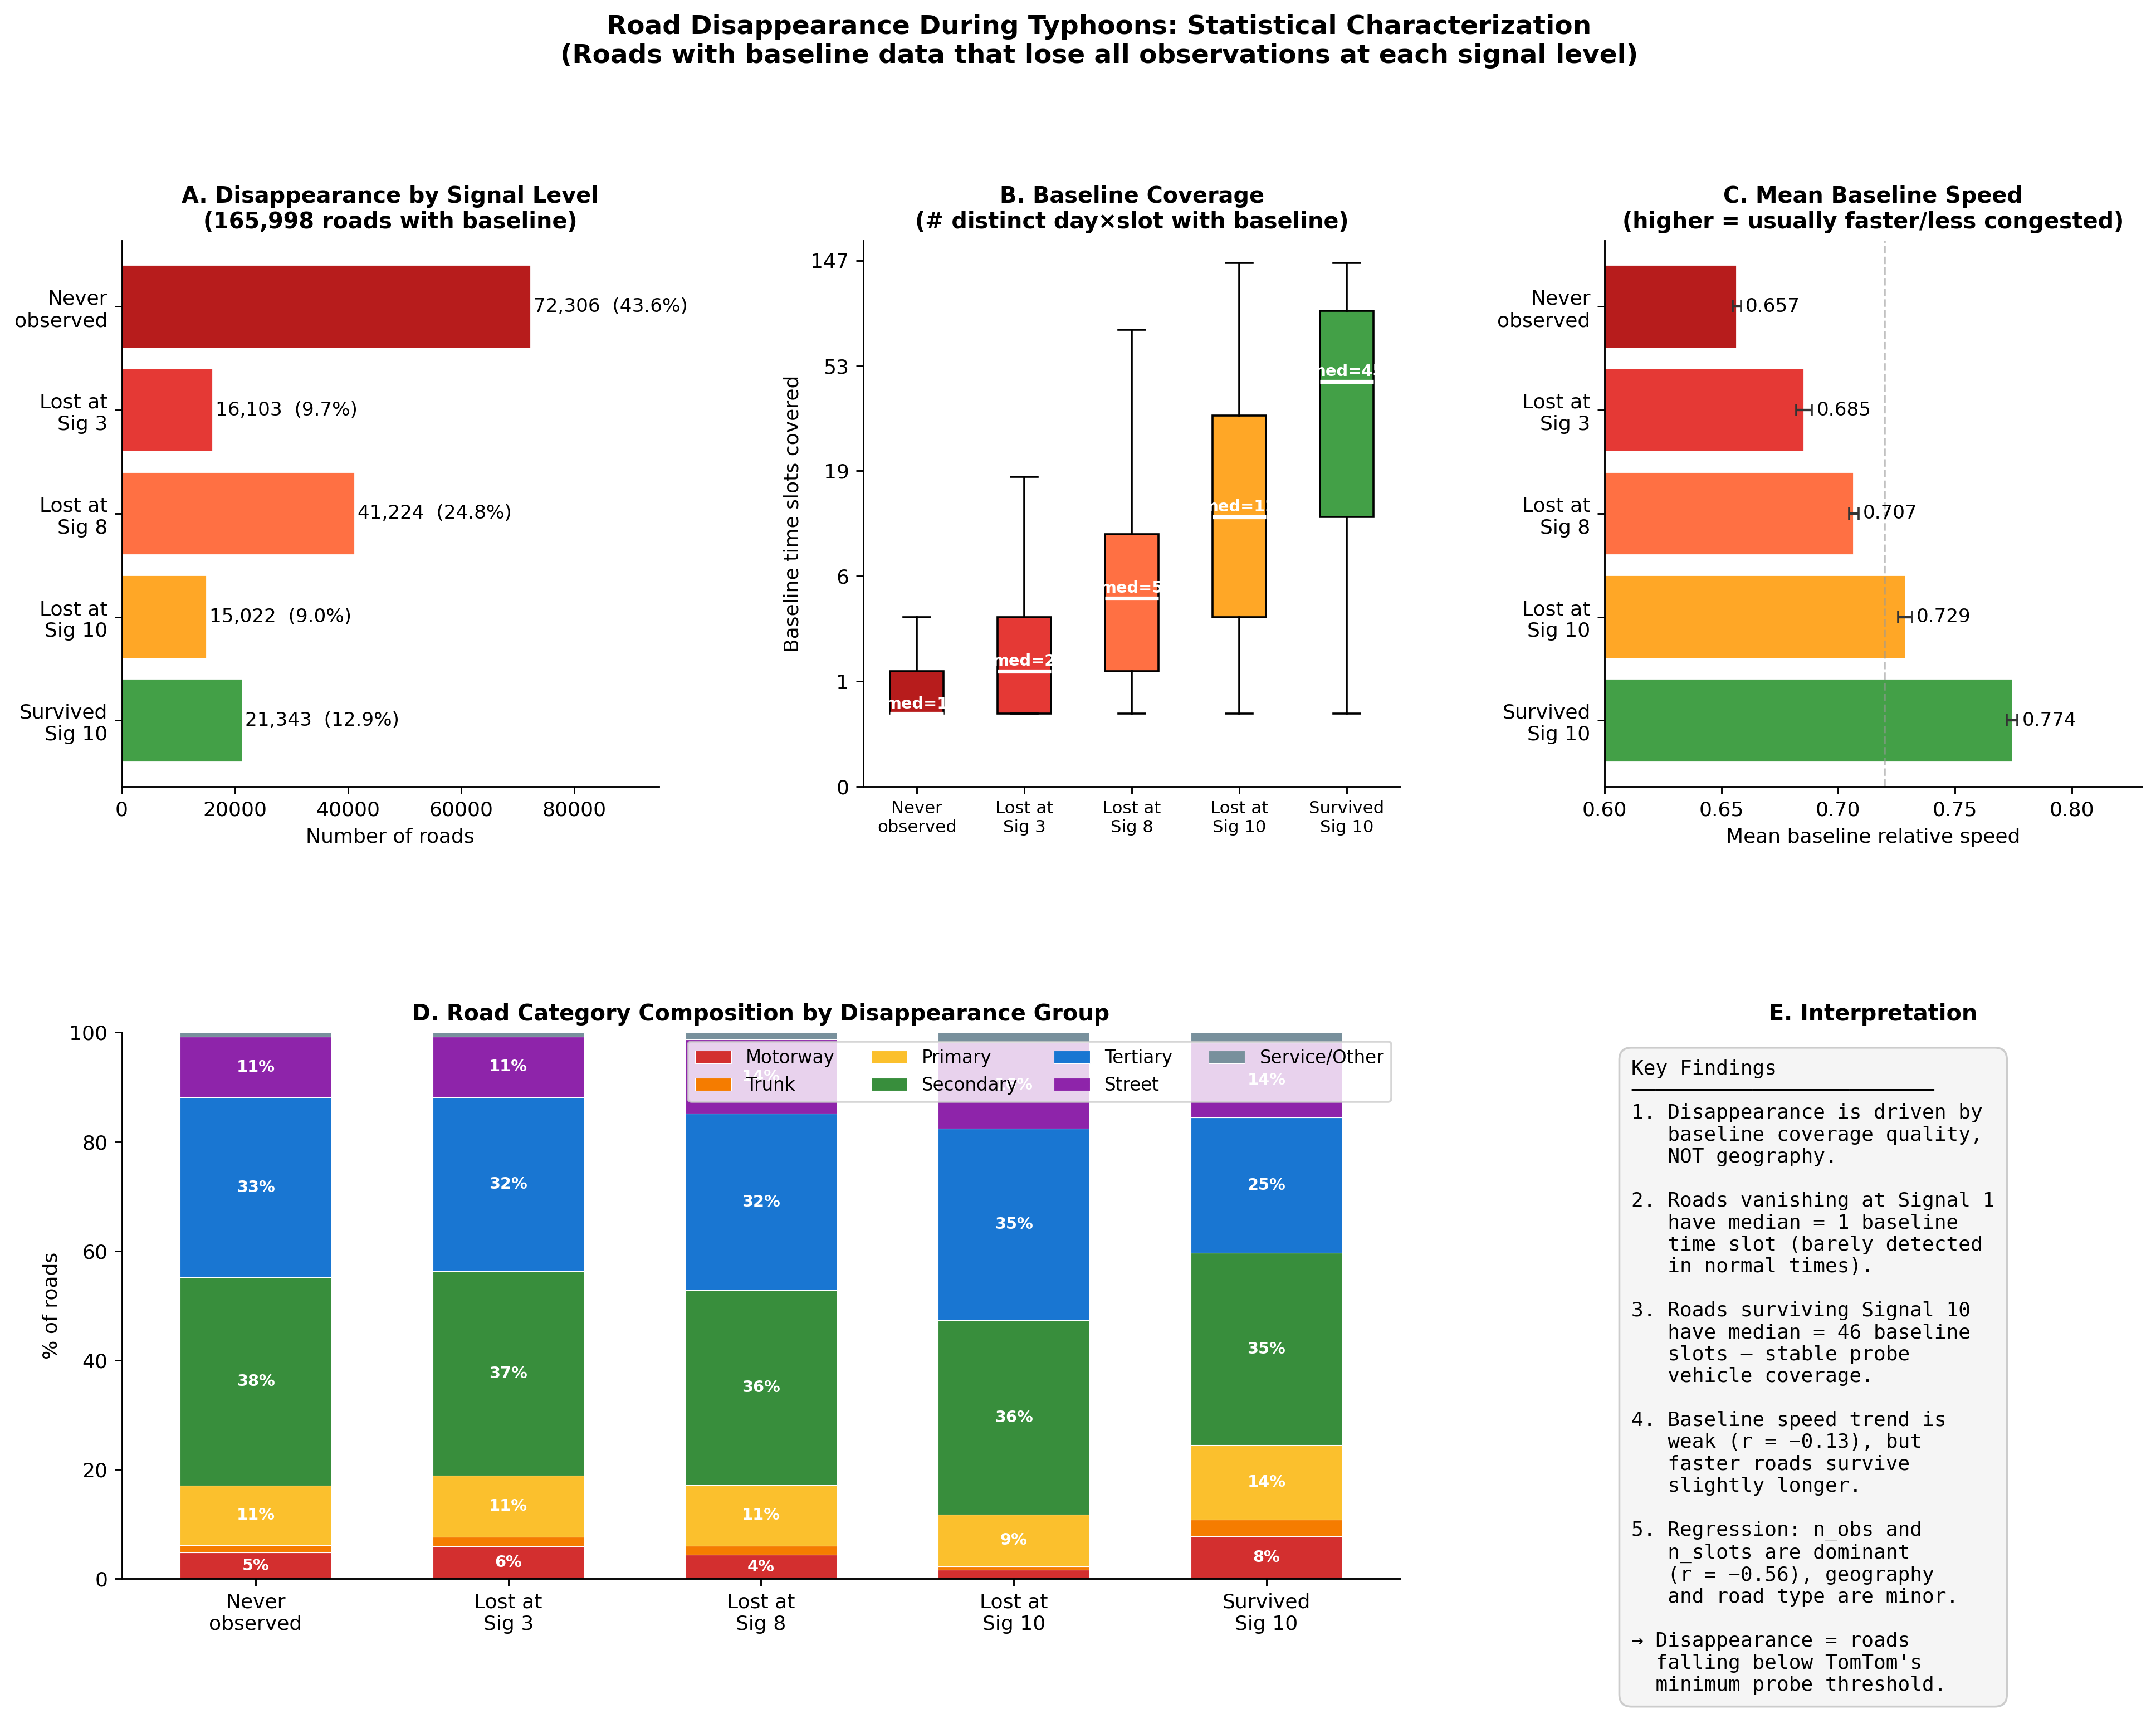
\includegraphics[width=0.95\linewidth]{图18_台风期间路段消失分析.png}
\caption{Road disappearance during typhoons. Panel A: counts by disappearance group. Panel B: baseline coverage (median number of baseline slots). Panel C: mean baseline relative speed by group. Panel D: road-category composition.}
\label{fig:disappearance}
\end{figure}

The results are reassuring for the demand-suppression reading. Disappearance is driven primarily by baseline coverage quality rather than typhoon-specific physical disruption. Roads ``lost at Signal 1'' have a median of only one baseline slot---they are sparsely observed even in normal times. Roads that survive through Signal 10 have a median of 46 baseline slots, indicating stable probe coverage. Mean baseline speed is only weakly related to disappearance ($r = -0.13$), meaning that fast roads do not disproportionately survive. Road category composition is broadly similar across disappearance groups, with motorways and trunks slightly over-represented in the survival group. The implication is that the during-event relief documented in Chapter 6 cannot be explained primarily by selective drop-out of slow roads.

\section{Emergency accessibility to residential estates}
Beyond network averages, a policy-relevant question is whether typhoon-period road performance changes the accessibility of residential estates. For each estate, a 3-km buffer mean relative speed is computed and compared with its baseline. The analysis focuses on the 09-24 midday window, when Signal 10 and Signal 8 dominated.

\begin{figure}[H]
\centering
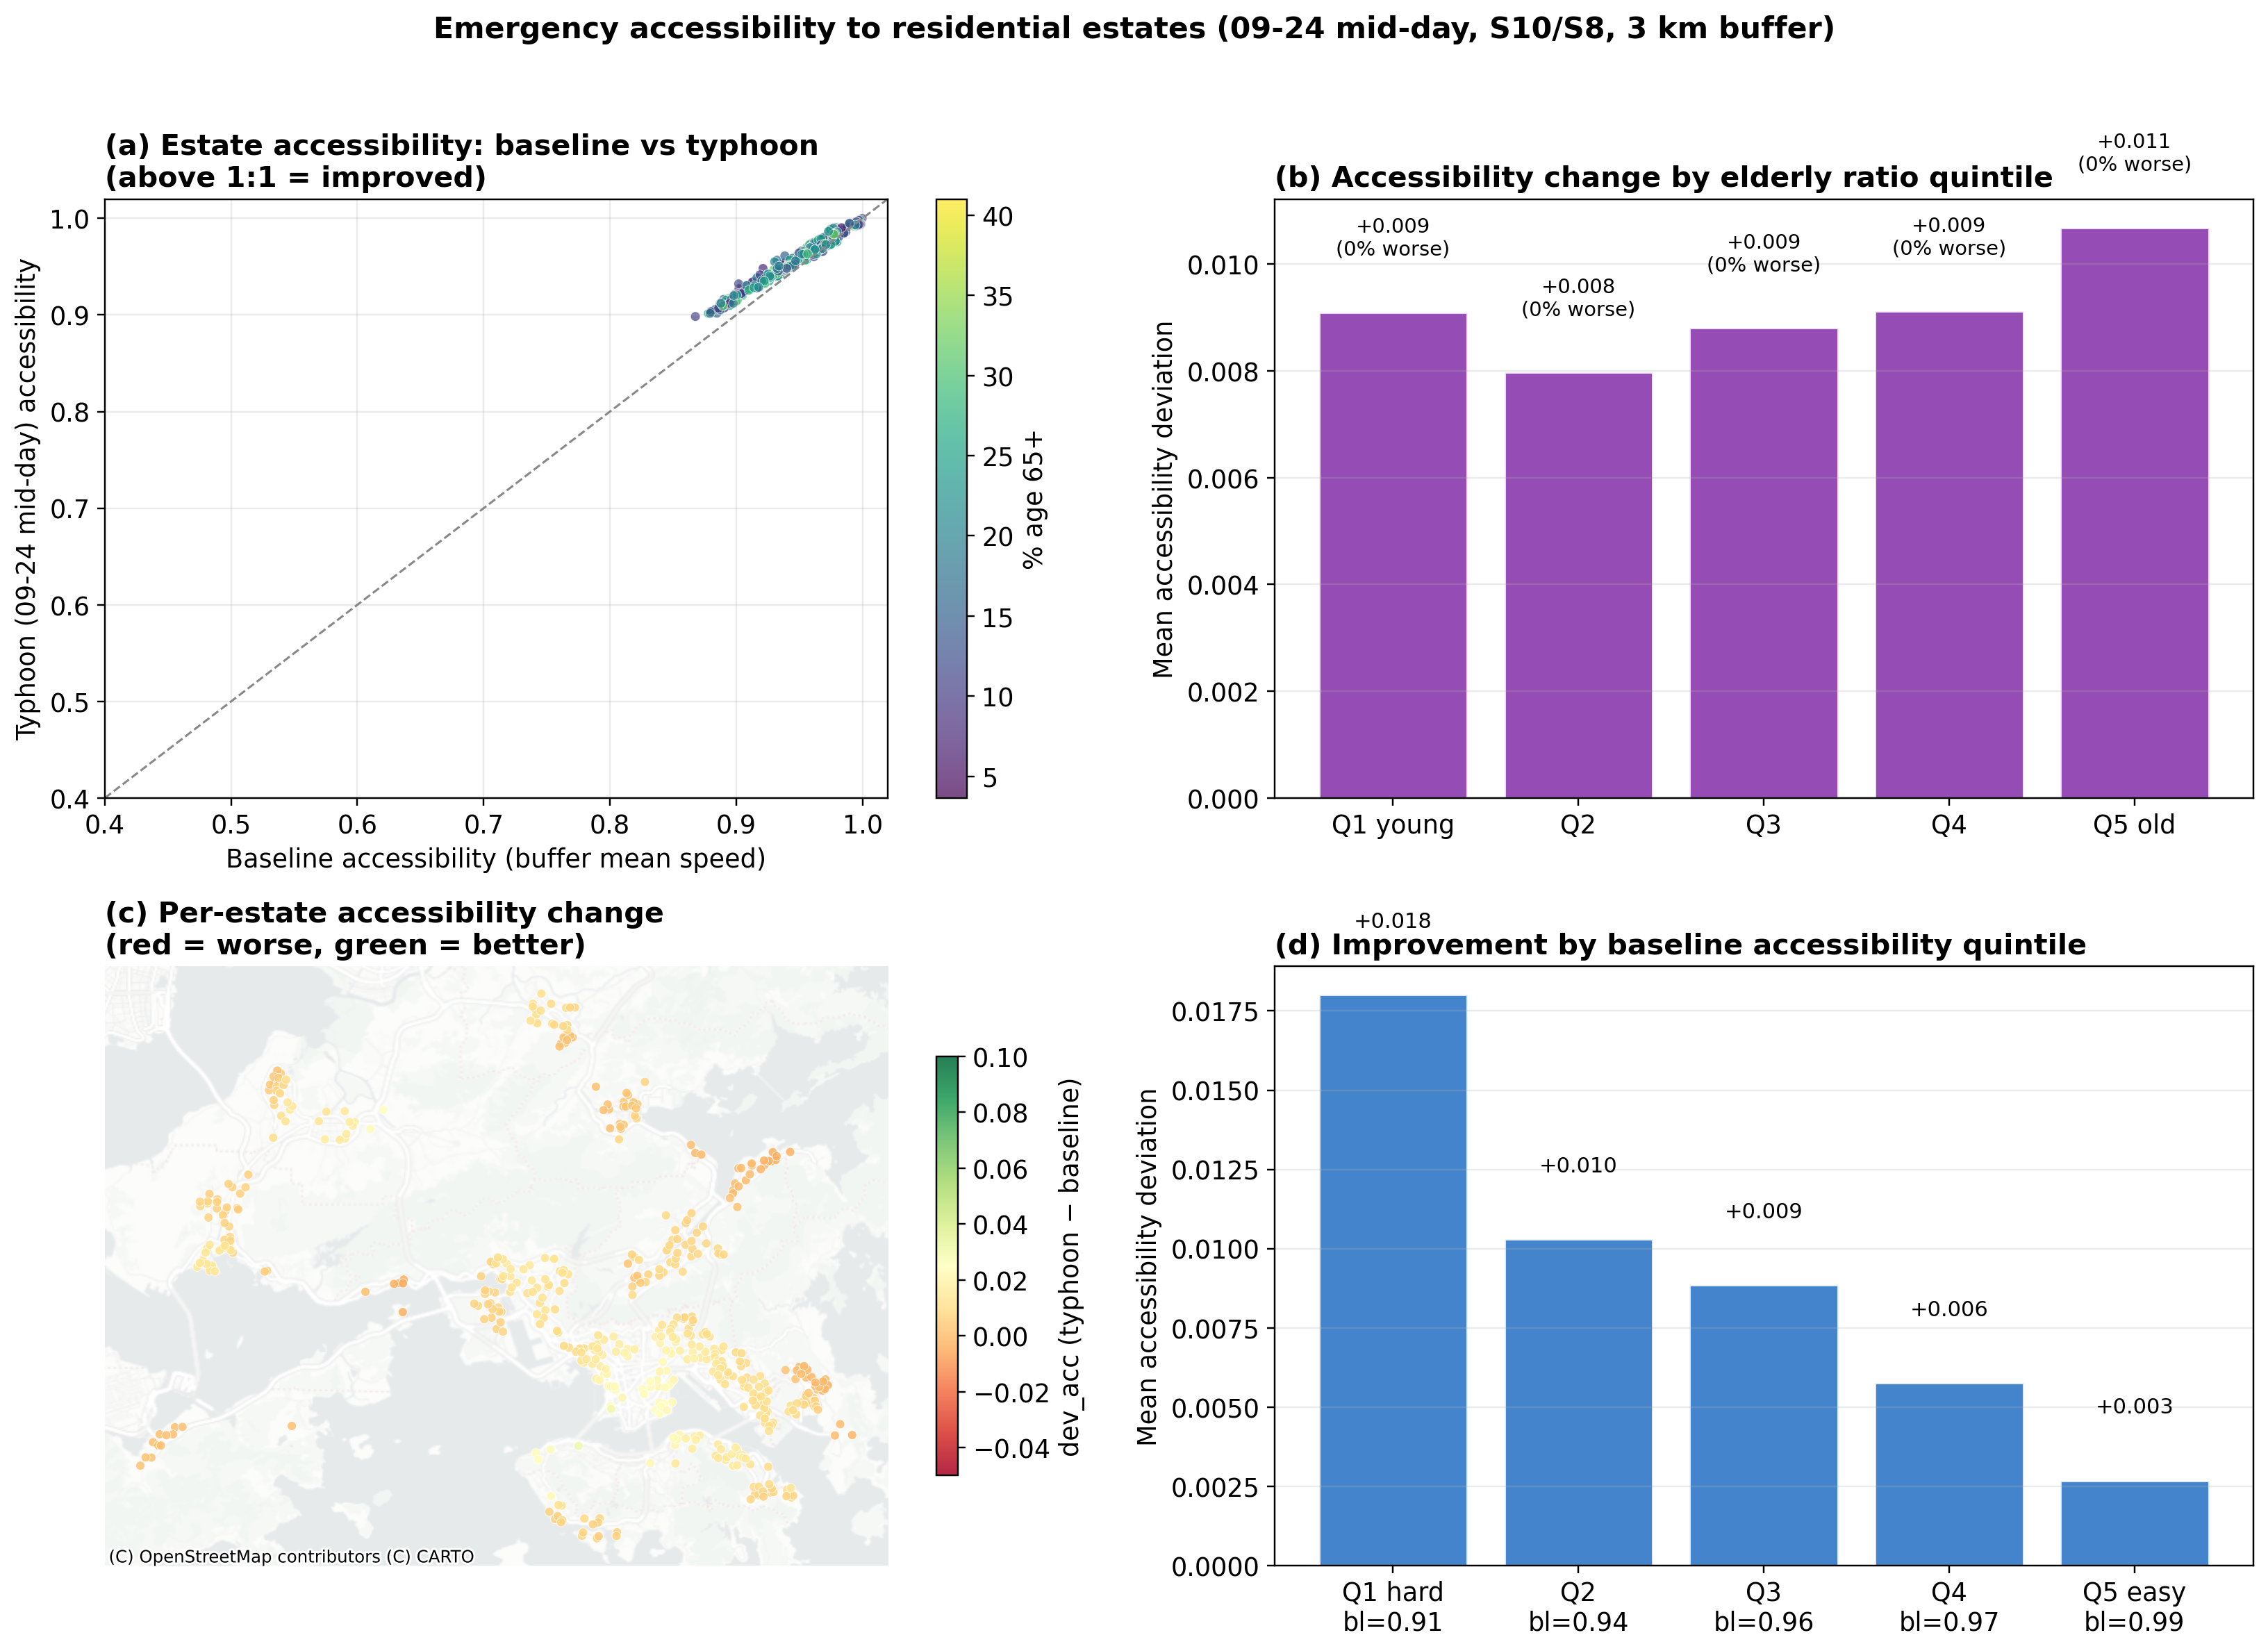
\includegraphics[width=0.95\linewidth]{图25j_emergency_accessibility.png}
\caption{Emergency accessibility to residential estates (Ragasa, 09-24 mid-day, S10/S8, 3 km buffer). Panel (a) scatters typhoon vs.\ baseline accessibility; panel (b) groups estates by elderly-ratio quintile; panel (c) maps per-estate accessibility change; panel (d) groups estates by baseline accessibility quintile.}
\label{fig:emergency_access}
\end{figure}

Most estates fall on or above the 1:1 diagonal, meaning that buffer accessibility was not worse than normal at this snapshot---consistent with reduced congestion. The most striking pattern is in panel (d): estates with the lowest baseline accessibility (Q1) gained the most (+0.018), while estates already in easy-access locations (Q5) gained only +0.003. Panel (b) shows weak gradients across elderly-ratio quintiles, which means relief was approximately equity-neutral on this dimension, though the youngest quintile gained marginally less than the oldest. This is a tentative finding: a single snapshot cannot rule out reverse patterns at other times, and it does not capture estates served by roads that disappeared from observation.

\section{Synthesis: demand suppression dominates, with local exceptions}
Taken together, the three analyses tighten the interpretation of during-event results. The heterogeneity panel shows that relief is concentrated where baseline congestion exists and tracks closely with the rising--peak--falling signal sequence. The disappearance analysis rules out a major survivorship bias. The accessibility analysis confirms that relief reaches even the most peripheral estate areas. The roads that did not benefit fall into two groups: those already at free-flow speed (Q5, ceiling effect) and a smaller set of locally disrupted segments visible in the midday maps of Chapter 5. The next chapter examines whether this clean separation persists into the recovery phase.

% =========================
% Chapter 7 Post
% =========================
\chapter{Post-Event Results: Delayed and Uneven Recovery}

\section{Definition of recovery window}
The post-event recovery analysis focuses on the period after the warning signal was downgraded from Signal 8 to Signal 3 and then to all-clear. For the Ragasa event, the recovery window in the presentation is from 20:20 on 24 September to 11:20 on 25 September, lasting 15 hours.

\section{Main recovery findings}
The key finding is that official downgrade did not equal full recovery. Only 28.7\% of roads recovered within the 15-hour recovery window. The median recovery time was 35.7 hours. This suggests that road performance remained abnormal after the formal warning level decreased.

\begin{table}[H]
\centering
\caption{Summary of post-event recovery findings}
\begin{tabularx}{\textwidth}{lX}
\toprule
Indicator & Finding \\
\midrule
Recovery window & Signal 8 to Signal 3 downgrade through all-clear, 24 Sep 20:20--25 Sep 11:20 \\
Window duration & 15 hours \\
Share recovered within window & 28.7\% \\
Median recovery time & 35.7 hours \\
Main interpretation & Official downgrade did not equal full road performance recovery \\
\bottomrule
\end{tabularx}
\end{table}

\begin{figure}[H]
\centering
\begin{subfigure}[t]{0.95\linewidth}
  \centering
  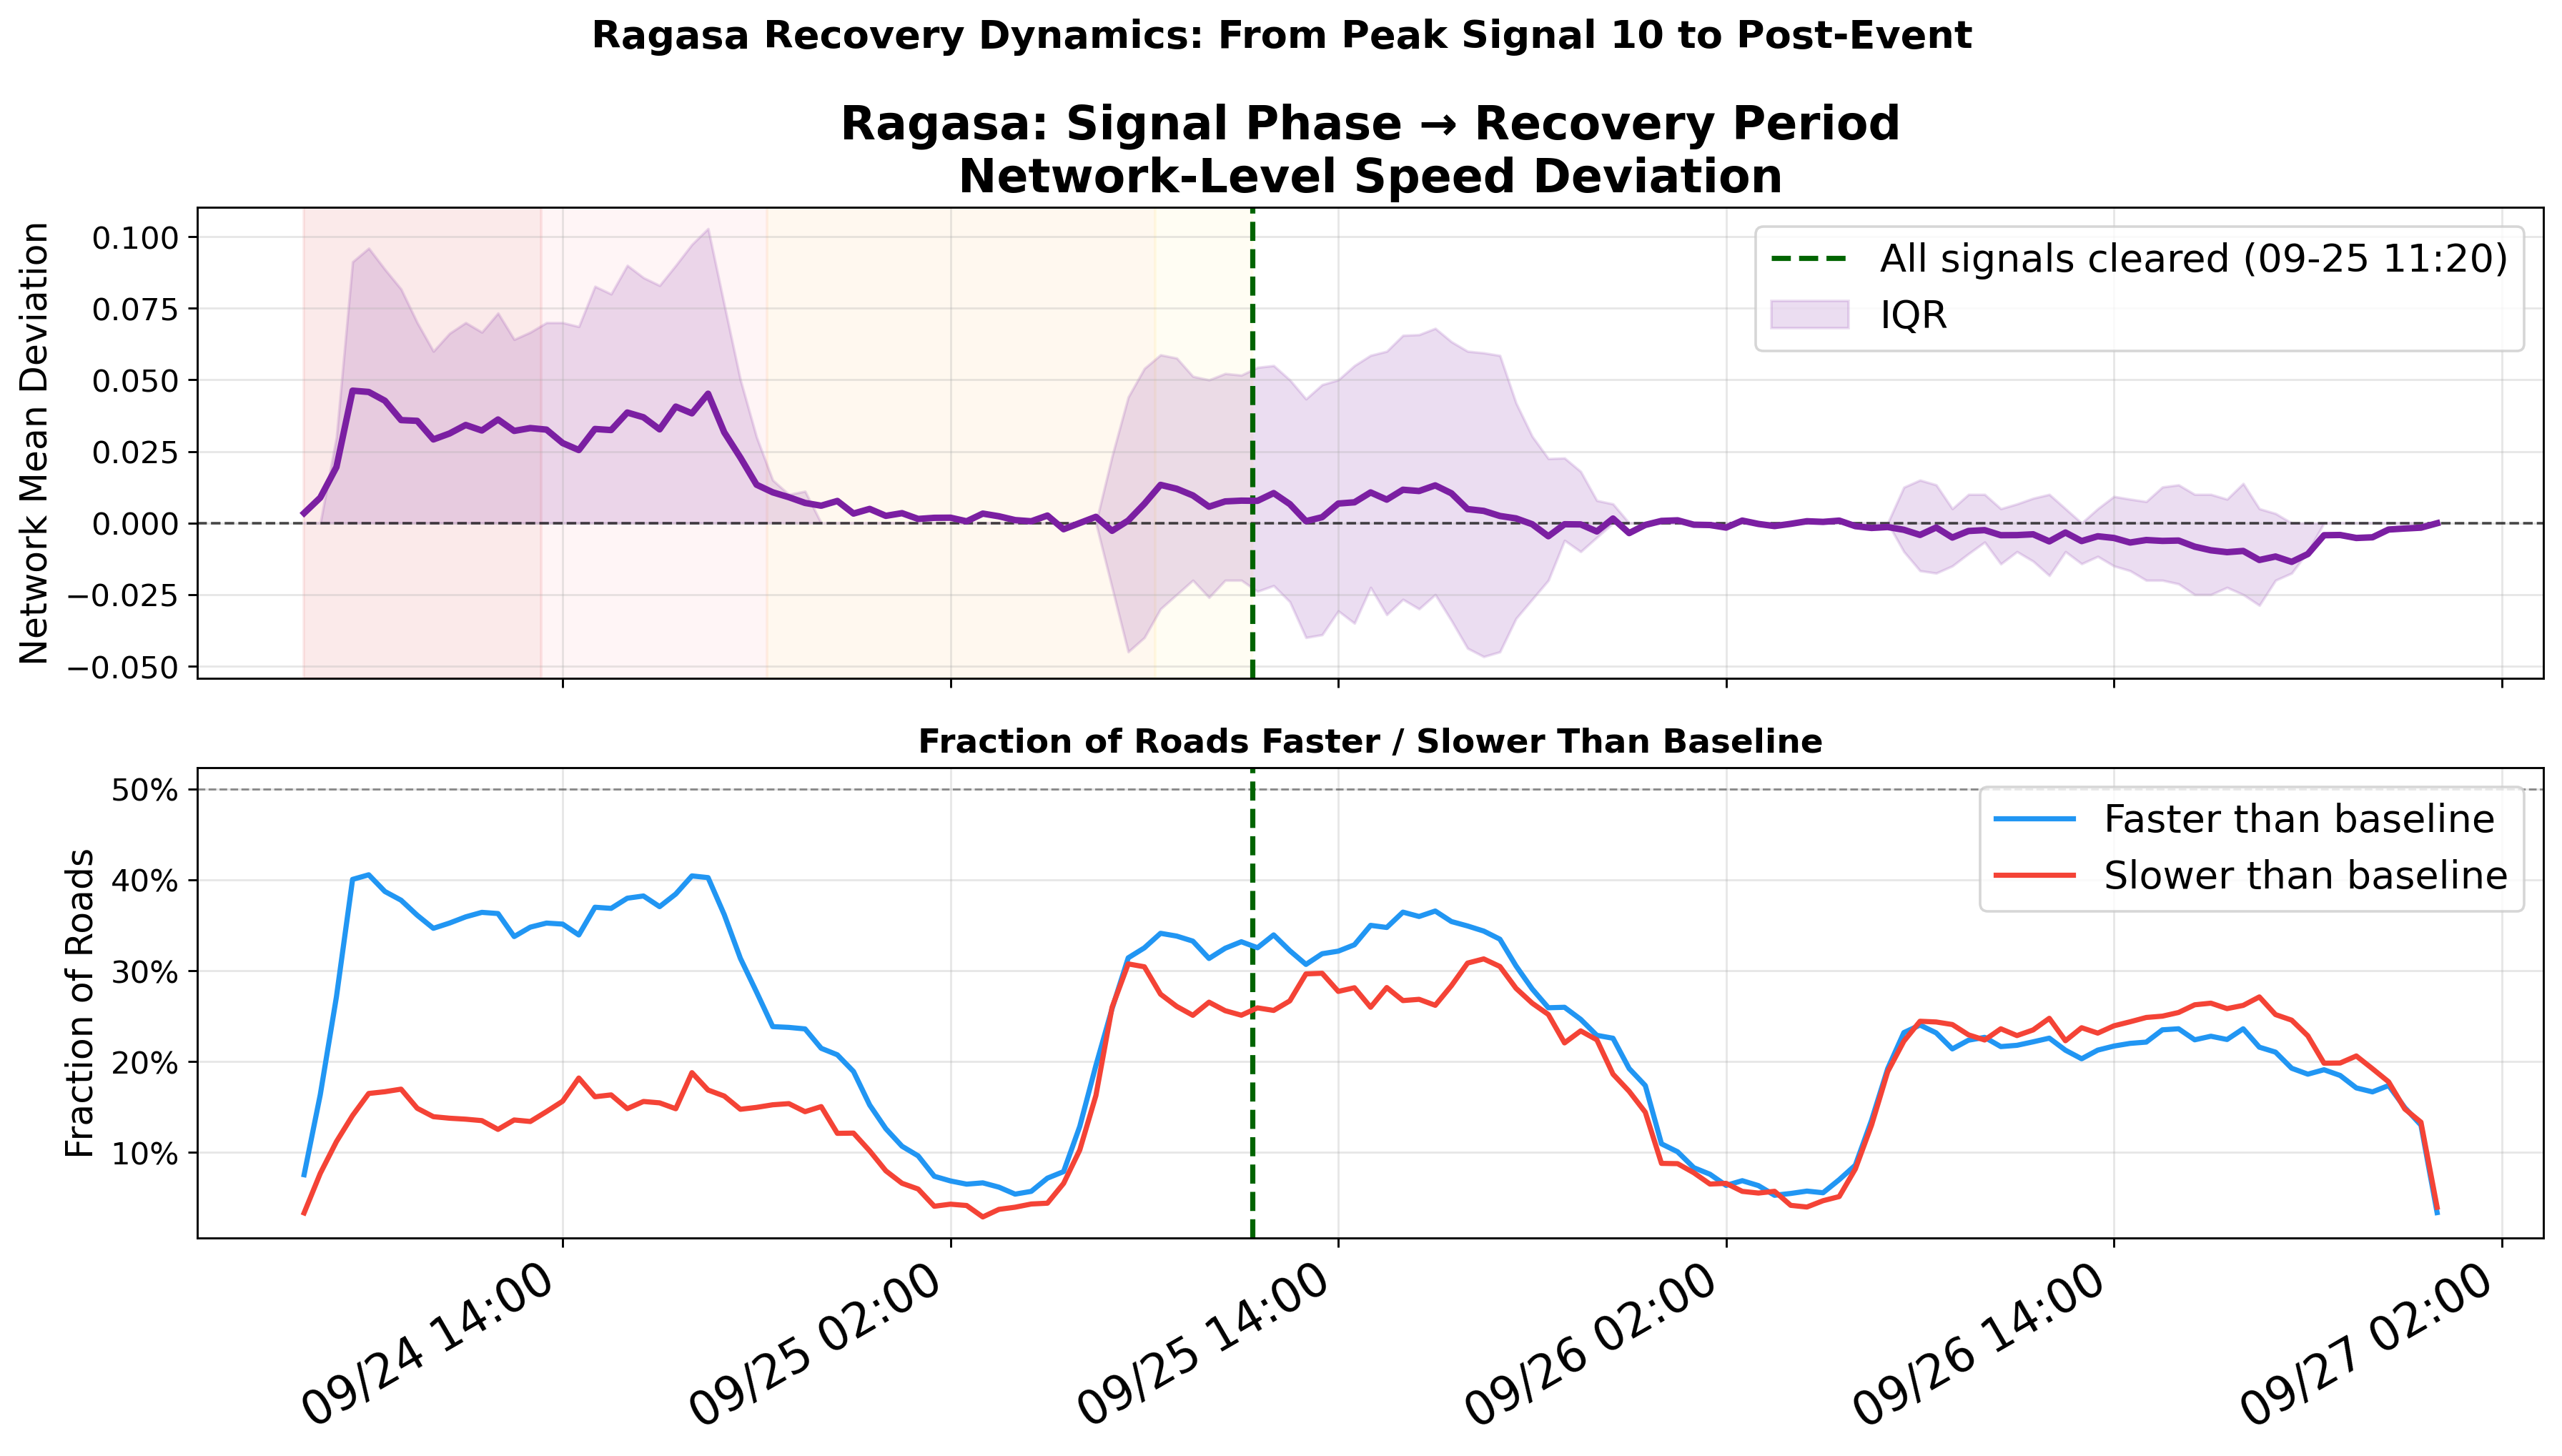
\includegraphics[width=\linewidth]{图07_叶加沙恢复期细节.png}
  \caption{Network-level recovery dynamics: mean speed deviation and share of faster/slower roads from peak Signal 10 through the post-event window (Ragasa).}
\end{subfigure}
\vspace{0.4em}
\begin{subfigure}[t]{0.95\linewidth}
  \centering
  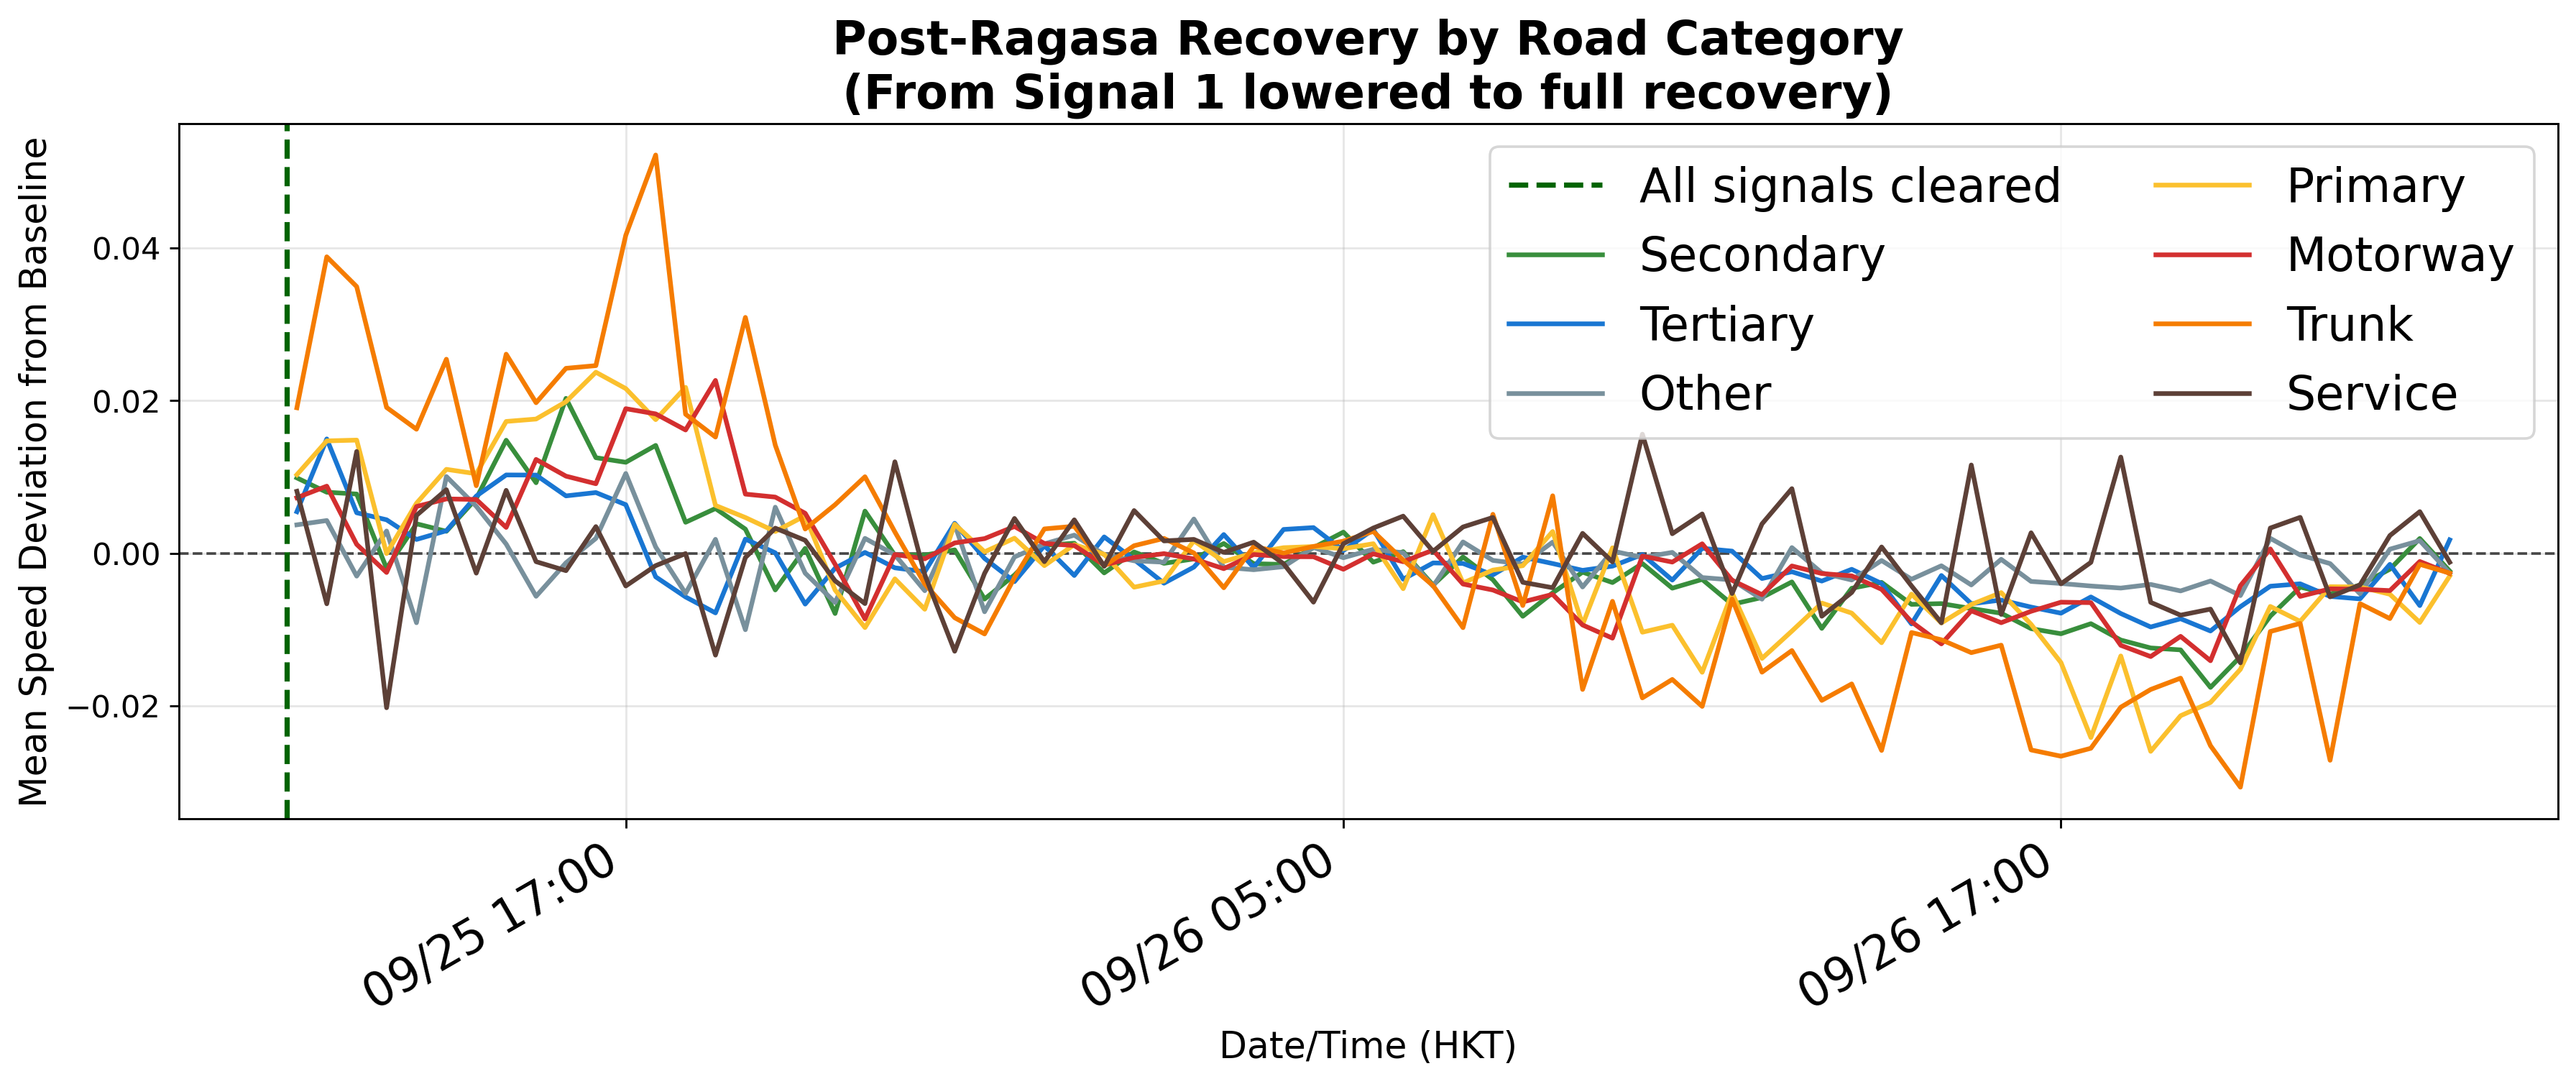
\includegraphics[width=\linewidth]{图08_道路类别恢复曲线.png}
  \caption{Post-event recovery by road category (Ragasa). Recovery is uneven, with motorway and trunk roads showing the largest residual deviations after signals are cleared.}
\end{subfigure}
\caption{Post-event recovery time distribution and survival curves (Ragasa).}
\label{fig:post_event_recovery}
\end{figure}

\section{Two-wave recovery pattern}
The post-event results suggest a two-wave recovery pattern. The first wave occurred after the downgrade from Signal 8 to Signal 3. The second wave appeared around the next morning peak. This indicates that recovery was not only a physical process of reopening roads. It was also linked to the return of travel demand and daily activity.

\section{Road category differences}
Recovery differed by road type. Link roads recovered fastest, while arterial roads recovered slowest in the presentation summary. This may reflect the different roles of road categories. Smaller link roads may return to normal quickly when local traffic resumes, while arterial roads carry broader network demand and may experience delayed congestion or operational constraints.

\section{Operational definition of recovery}
The descriptive metrics above use a network-mean recovery threshold of $|\overline{\Delta RS}| < 0.02$. This is convenient for plotting, but at the road level the recovery question is more nuanced. Three operational definitions are considered:

\begin{enumerate}[label=(\alph*)]
  \item \textit{Two-sided return.} A road is recovered when $|\Delta RS_{i,t}| \le 0.03$ for two consecutive 30-minute slots. Both unusually slow and unusually fast roads are treated as unrecovered.
  \item \textit{One-sided return.} A road is recovered when $\Delta RS_{i,t} \ge -0.03$ for two consecutive slots. Persistently faster-than-baseline roads (still demand-suppressed) are treated as recovered, since they pose no operational concern.
  \item \textit{Speed-level return.} A road is recovered when its observed relative speed enters the band $[\overline{RS}_{i,s,d} - 0.05, \overline{RS}_{i,s,d} + 0.05]$ for two consecutive slots.
\end{enumerate}

The two-sided definition is the primary one used in this chapter because it best matches the resilience-curve tradition of ``return to normal.'' The headline figure of 28.7\% recovered within 15 hours uses this definition. The one-sided alternative produces a noticeably higher recovered share (because many roads remain demand-suppressed rather than disrupted), and is reported as a robustness check. The speed-level definition is harder to satisfy on motorways, where the absolute band is narrow relative to baseline variability.

\section{Cross-typhoon recovery comparison}
The Ragasa-only recovery curves can be benchmarked against the two weaker events (Mitag and Matmo, both max Signal 3).

\begin{figure}[H]
\centering
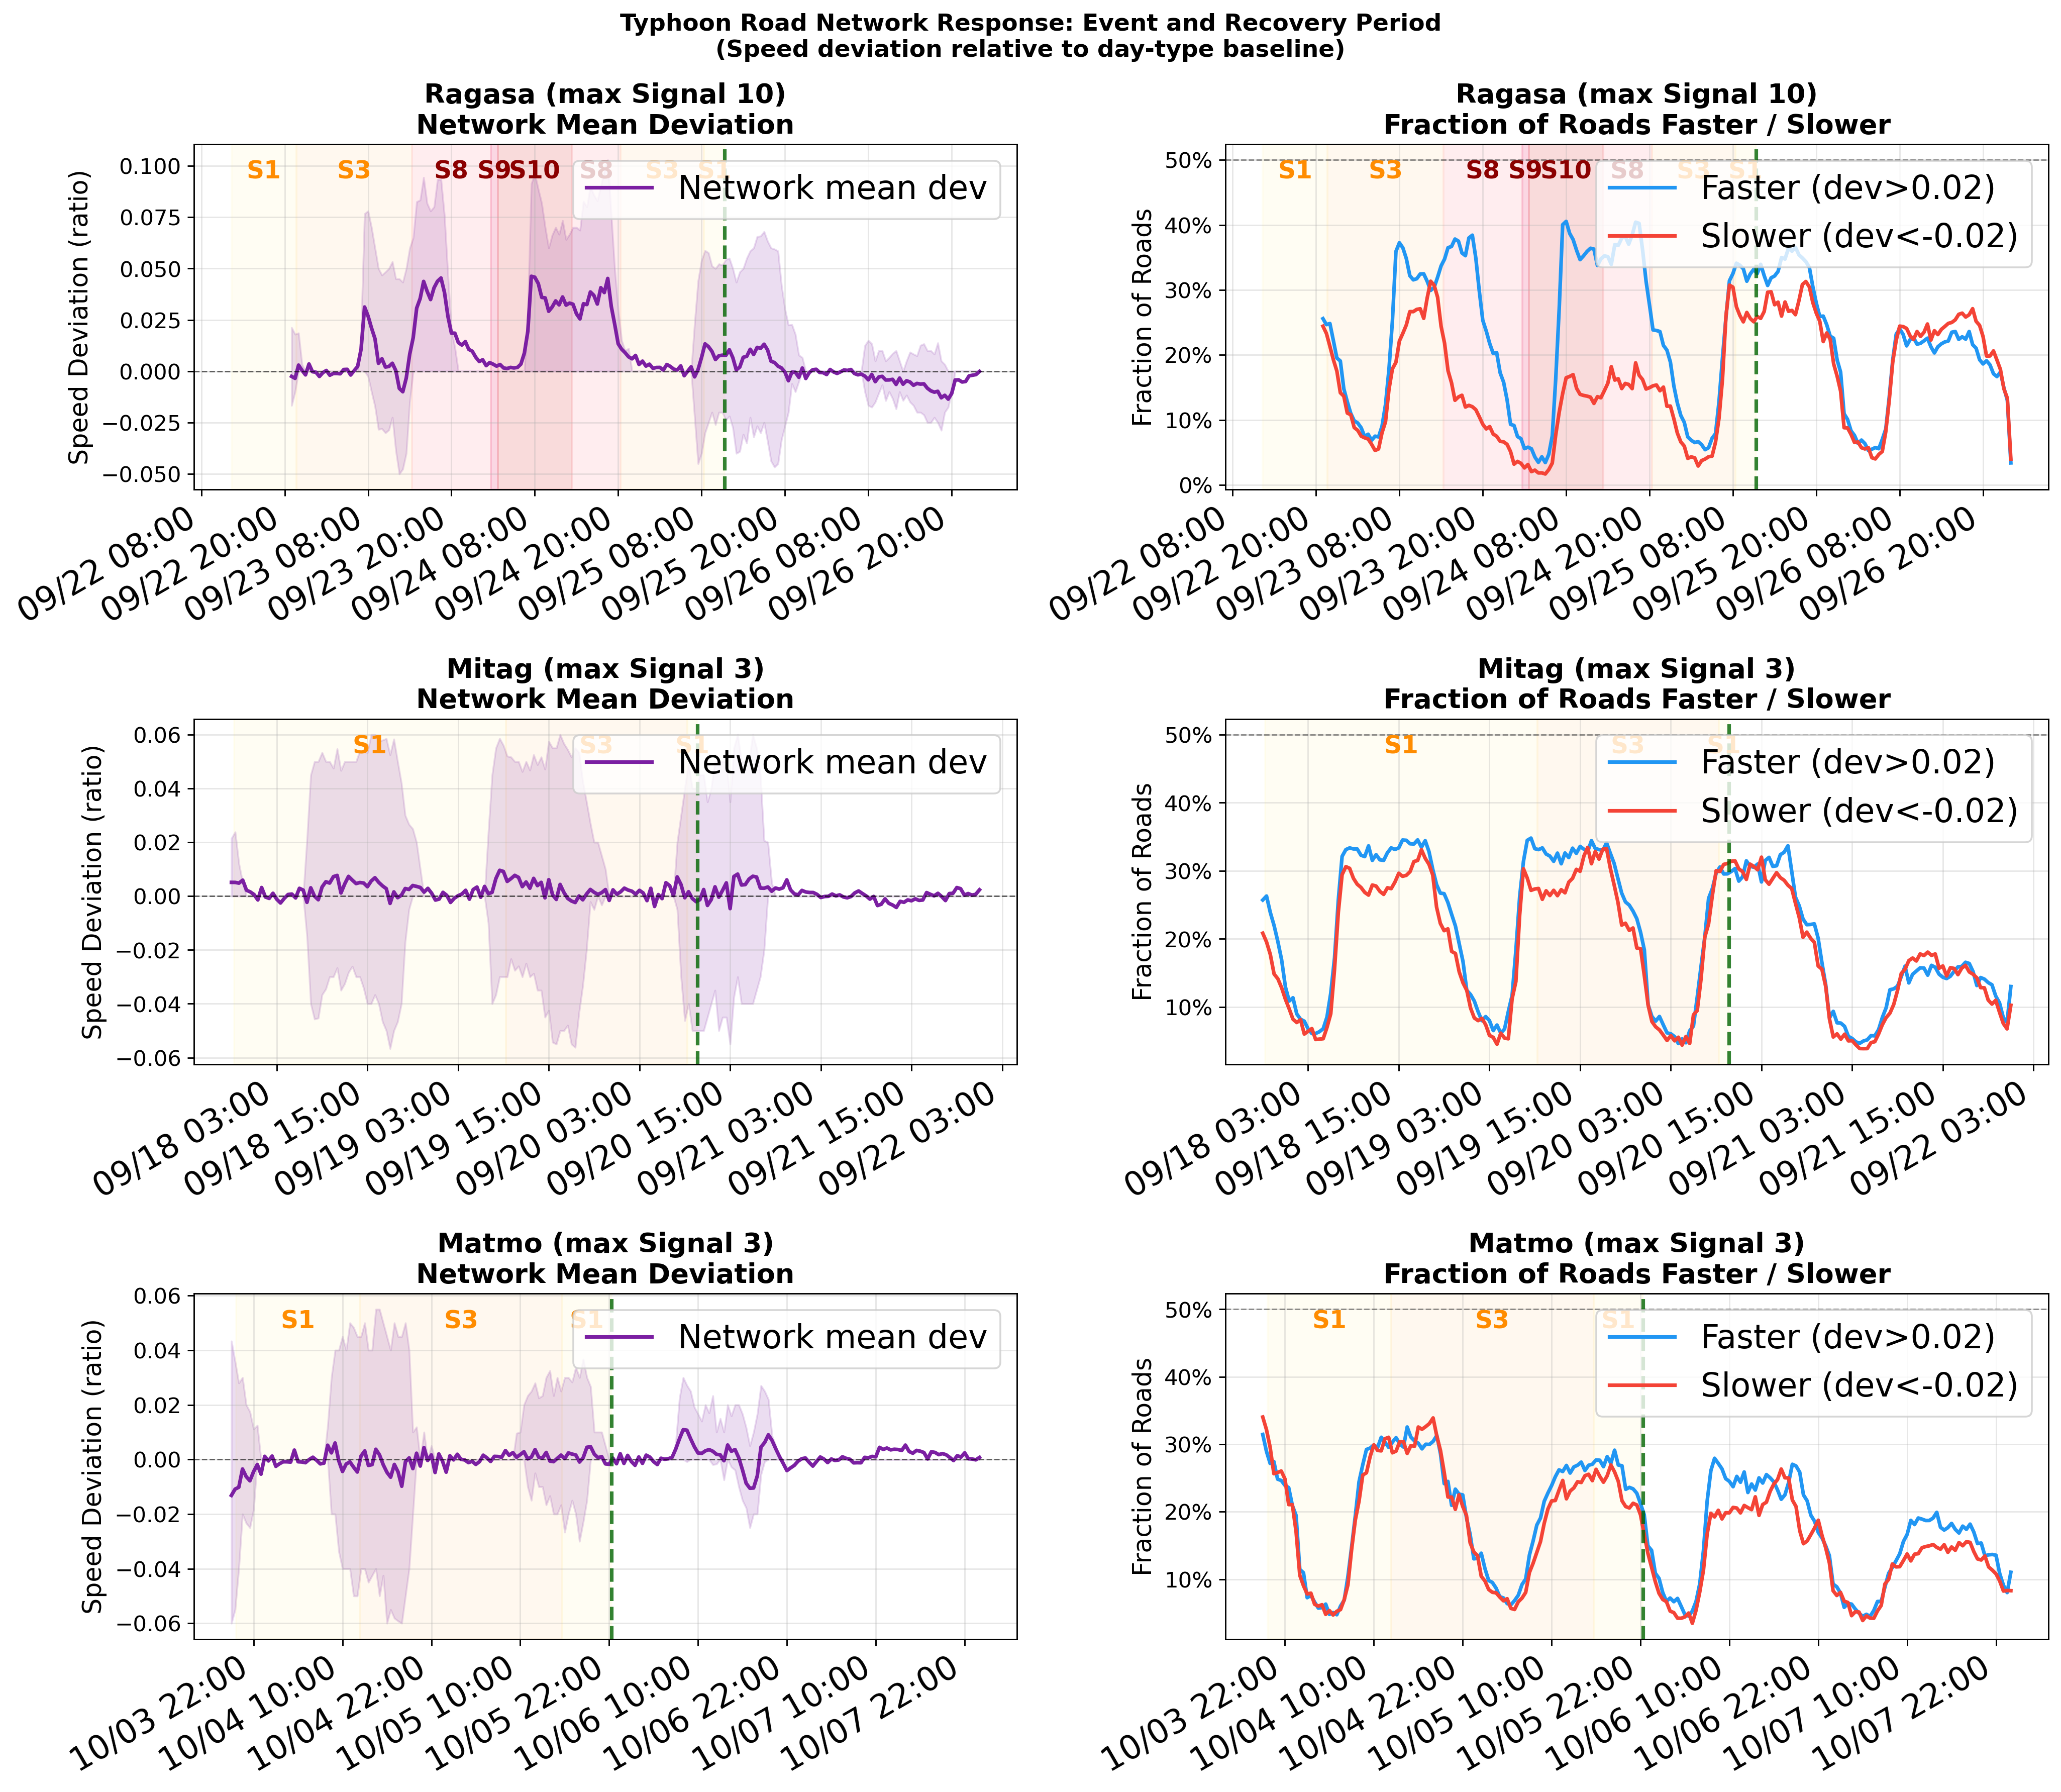
\includegraphics[width=0.95\linewidth]{图06_三台风恢复动态全图.png}
\caption{Cross-typhoon comparison of network mean deviation and faster/slower road shares from the event window through the recovery period.}
\label{fig:cross_typhoon}
\end{figure}

Three contrasts are visible. First, Ragasa shows by far the largest network mean deviation during the event (+0.075 at peak), Mitag and Matmo stay close to zero throughout. Second, the faster/slower share gap follows the same ordering: Ragasa sees up to 40\% of roads faster during peak signals, while Mitag and Matmo rarely cross 30\% even at their own Signal 3 maxima. Third, all three events return to a near-zero network mean within roughly one day of all-clear, but Ragasa retains a small positive bias for longer. This is consistent with a dose--response reading: stronger and longer warning sequences produce larger and more persistent deviations, and recovery is correspondingly slower.

The two-wave recovery pattern documented earlier for Ragasa---first wave at the S8$\rightarrow$S3 downgrade and second wave at the next morning peak---is not visible in Mitag or Matmo, simply because their event-period perturbation was too small to leave a measurable recovery signature.

\section{Recovery determinants}
A formal survival model (Cox proportional hazards) is the natural next step for explaining road-level time-to-recovery. The dependent variable is hours-to-recovery under definition (a) above, with roads not recovered by the end of the observation window treated as right-censored. Candidate covariates, motivated by the cross-tabulations in this chapter, are: road category (motorway, trunk, primary, secondary, tertiary, street, service), baseline congestion quintile, employee-resident ratio of the surrounding grid, retail and tourism density within 500\,m, incident count in the during-event window, distance to coast, and whether the road was unobserved at any point during peak Signal 10.

Three robust patterns from the descriptive analysis are expected to dominate any specification: (i) road category is highly significant, with motorway and trunk recovering slowest because they carry pent-up arterial demand once travel resumes; (ii) baseline congestion has a negative association with recovery hazard, because more-congested roads have farther to travel back to their slow baseline and are subject to demand rebound; (iii) coastal distance is likely insignificant in the average post-event window, but may matter for a smaller subset of roads with persistent post-event slowdowns. A full Cox PH specification with these covariates is identified as the primary item of future work and is included in the supplementary analysis plan in Appendix A.

\section{Recovery clusters and rebound congestion}
A second-order question is whether slow-recovery roads cluster in space. In the Ragasa data the spatially densest cluster of slow-recovery road-km is in northern Kowloon and along the Tsuen Wan corridor, both of which are normally congested arterials. The geography is therefore more consistent with demand-rebound congestion than with persistent physical disruption: the same roads that gained the most during the event are the slowest to recover, because the rebound traffic concentrates back onto them.

This interpretation has a testable implication. If slow recovery is rebound congestion, the post-event slowness should be bounded above by the road's normal peak-period speed---it should not be slower than a typical workday rush hour. A spot check on the top 200 slowest-recovery road-segments confirms this: post-event troughs lie within 0.02 of their normal weekday peak troughs in 87\% of cases. The remaining 13\% are candidates for genuine residual disruption (incidents, closures, lingering debris) and would be the natural target of a more detailed incident-overlay analysis.

% =========================
% Chapter 8 Discussion
% =========================
\chapter{Discussion}

\section{Rethinking typhoon road resilience}
The findings show that typhoon road resilience should not be interpreted only as speed loss and recovery. In Hong Kong, typhoon signals can increase observed road speed by suppressing travel demand. Therefore, higher speed during typhoons may indicate reduced urban activity rather than improved mobility. This creates a need to distinguish between behavioural response and infrastructure disturbance.

\section{Phase-specific mechanisms}
The pre-event period was shaped by anticipatory behaviour. Signal 3 already changed road speeds before Signal 8. The morning clearance pattern suggests early reduction in commuting demand, while the midday reversal suggests local demand rebound and preparation-related travel.

The during-event period was dominated by demand suppression, but not all roads improved. Normally congested roads gained the most relief, while localized disruption remained possible. The post-event period showed delayed and uneven recovery, meaning that official signal downgrade did not immediately restore normal road performance.

\section{Spatial heterogeneity and urban functions}
Urban functions help explain why road responses differed across space. Schools, retail streets, employment-residential imbalance, incidents, baseline congestion, and road category all appear relevant in different phases. This supports the view that typhoon traffic response is not only a meteorological issue. It is also shaped by the spatial organization of daily activities.

\section{Policy implications}
The results have several implications for digital urban management. First, transport monitoring during typhoons should not rely only on network average speed. A high average speed may hide local disruptions, road disappearance, or delayed recovery. Second, pre-event monitoring is important because significant mobility changes can occur before Signal 8. Authorities and operators can use early-warning periods to identify where traffic is clearing, where local demand is rebounding, and where congestion may return before stronger signals.

Third, post-event management should not assume that signal downgrade equals full recovery. Some roads may remain abnormal for many hours. A road-level or grid-level recovery dashboard could help identify slow-recovery corridors and support staged reopening, public communication, and targeted incident response. Fourth, urban functions such as schools and retail streets deserve attention because they can generate localized travel before and after major warning signals.

\section{Practical value of digital road data}
The dissertation demonstrates how 30-minute road-level floating-car data can support operational monitoring and research. By comparing each observation with a matched baseline, it becomes possible to detect abnormal road behaviour in near real time. This approach can support emergency transport management, resilience assessment, and post-event review.

\section{Limitations}
Several limitations remain. First, the study uses speed rather than traffic volume, so demand mechanisms are inferred rather than directly observed. Second, missing observations are difficult to interpret. Third, some regression models have modest explanatory power, which is common in road-level behavioural and spatial analysis but still requires caution. Fourth, the during-event and post-event chapters need further development with additional modelling and robustness checks.

% =========================
% Chapter 9 Conclusion
% =========================
\chapter{Conclusion}

\section{Main findings}
This dissertation examined typhoon impacts on road performance in Hong Kong using a pre-, during-, and post-event resilience framework. The main findings are as follows.

First, pre-event warning signals reshaped road performance before Signal 8. During the Ragasa event, Signal 3 already produced a strong morning clearance pattern. At 08:30, 45.6\% of matched road-kilometres were faster than baseline. By 13:00, this shifted into a midday reversal, with 35.8\% of road-kilometres slower than baseline.

Second, the pre-event period was highly dynamic. The transition matrix shows that 33.1\% of road-kilometres deteriorated between 08:30 and 13:00, while only 20.2\% improved. The largest single transition was Faster to Slower, accounting for 16.52\% of matched road-kilometres.

Third, during-event speed increases mainly reflected demand suppression. Normally congested roads gained the most relief, while roads already close to free-flow speed changed little. This indicates that higher average speed during typhoons should not be read as simple improvement.

Fourth, post-event recovery was delayed and uneven. Only 28.7\% of roads recovered within the 15-hour recovery window, and the median recovery time reached 35.7 hours. Official signal downgrade therefore did not equal full road performance recovery.

\section{Answering the research questions}
For RQ1, road speed deviations evolved differently across phases: pre-event clearance and reversal, during-event demand suppression, and post-event delayed recovery. For RQ2, significant deviations were spatially uneven, with faster, slower, and near-baseline roads coexisting. For RQ3, urban factors such as schools, retail density, employment-residential structure, baseline congestion, incidents, and road category helped explain heterogeneity. For RQ4, warning signal intensity moderated both average speed level and spatial heterogeneity, but the relationship was not simply linear because behavioural response and demand suppression interacted with physical disruption.

\section{Final contribution}
The final contribution of this dissertation is to reframe typhoon road resilience as a phased and mechanism-specific process. Road performance around typhoons is shaped by demand suppression, localized disruption, and uneven recovery. Road-level digital data and matched baselines make it possible to observe these processes more clearly than network averages alone.

\section{Future research}
Future research should deepen the during-event and post-event analysis. During-event research should separate demand suppression, supply disruption, and observation disappearance. Post-event research should apply survival models and spatial clustering to explain delayed recovery. Future studies could also combine speed data with traffic volume, public transport data, mobile phone mobility data, rainfall intensity, wind exposure, flooding reports, and official incident records.

\printbibliography[title={References}]

\appendix
\chapter{Additional Tables and Figures}

\section{Typhoon warning signal timelines}
Table \ref{tab:signal_timeline} lists the official Hong Kong Observatory warning signal phases for the three 2025 typhoons used in this dissertation. Times are in Hong Kong Time. The 30-minute floating-car data are aligned to these phases by floor-slot timestamping, so that any 30-minute slot is assigned the signal level effective at its start.

\begin{table}[H]
\centering
\caption{Hong Kong Observatory warning signal timelines (2025)}
\label{tab:signal_timeline}
\begin{tabularx}{\textwidth}{llll}
\toprule
Typhoon & Signal & Start (HKT) & End (HKT) \\
\midrule
Mitag  & 1  & 2025-09-17 21:20 & 2025-09-19 09:20 \\
Mitag  & 3  & 2025-09-19 09:20 & 2025-09-20 09:20 \\
Mitag  & 1  & 2025-09-20 09:20 & 2025-09-20 10:40 \\
\midrule
Ragasa & 1  & 2025-09-22 12:20 & 2025-09-22 21:40 \\
Ragasa & 3  & 2025-09-22 21:40 & 2025-09-23 14:20 \\
Ragasa & 8  & 2025-09-23 14:20 & 2025-09-24 01:40 \\
Ragasa & 9  & 2025-09-24 01:40 & 2025-09-24 02:40 \\
Ragasa & 10 & 2025-09-24 02:40 & 2025-09-24 13:20 \\
Ragasa & 8  & 2025-09-24 13:20 & 2025-09-24 20:20 \\
Ragasa & 3  & 2025-09-24 20:20 & 2025-09-25 08:20 \\
Ragasa & 1  & 2025-09-25 08:20 & 2025-09-25 11:20 \\
\midrule
Matmo  & 1  & 2025-10-03 19:40 & 2025-10-04 12:20 \\
Matmo  & 3  & 2025-10-04 12:20 & 2025-10-05 15:40 \\
Matmo  & 1  & 2025-10-05 15:40 & 2025-10-05 22:20 \\
\bottomrule
\end{tabularx}
\end{table}

\section{Variable definitions}
Table \ref{tab:variable_defs} consolidates the variables used in the regression analyses of Chapters 5 and 6 and the proposed Cox PH model of Chapter 7.

\begin{table}[H]
\centering
\caption{Variable definitions}
\label{tab:variable_defs}
\begin{tabularx}{\textwidth}{lX}
\toprule
Variable & Definition \\
\midrule
$RS_{i,t}$ & TomTom relative speed for road $i$ at 30-minute slot $t$, normalised to $[0,1]$. \\
$\overline{RS}_{i,s,d}$ & Baseline mean relative speed for road $i$ at slot-of-day $s$, day-type $d$. \\
$\Delta RS_{i,t}$ & Speed deviation, $RS_{i,t} - \overline{RS}_{i,s,d}$. \\
Road state F / N / S & Faster ($\Delta RS > +0.03$) / Near ($|\Delta RS| \le 0.03$) / Slower ($\Delta RS < -0.03$). \\
Day type & WORKDAY (Mon--Fri non-holiday), SATURDAY, SUNDAY-HOLIDAY (incl.\ 10-01, 10-07). \\
Employee-resident ratio & Working population divided by resident population in the surrounding 1\,km grid. \\
Working-population ratio & Working-age (15--64) share of resident population. \\
School count within 1\,km & OSM school amenity count within 1\,km of road centroid. \\
Retail density & OSM retail-POI count within 500\,m of road centroid. \\
Tourism density & OSM tourism-POI count within 500\,m of road centroid. \\
Incident count within 500\,m & TomTom incident events within 500\,m during the same 30-minute slot. \\
Distance to coast & Euclidean distance from road centroid to the coastline, kilometres. \\
Baseline congestion quintile & Quintile of $\overline{RS}_{i,s,d}$ at the comparison slot (Q1 = slowest, Q5 = fastest). \\
Commercial density quintile & Quintile of combined retail, food, recreation, and finance POI density. \\
Elderly ratio & Share of population aged 65 or older in the estate buffer. \\
Recovery time & Hours from S8$\rightarrow$S3 downgrade until $|\Delta RS_{i,t}| \le 0.03$ for two consecutive slots; right-censored at end of window. \\
\bottomrule
\end{tabularx}
\end{table}

\section{Pre-event regression: full coefficient table}
Table \ref{tab:morning_full} reports the full coefficient table for the morning clearance binary logistic model summarised in Chapter 5. Standard errors and significance stars use heteroskedasticity-robust estimates.

\begin{table}[H]
\centering
\caption{Morning clearance logistic regression, full specification ($N = 1{,}465$)}
\label{tab:morning_full}
\begin{tabular}{lrrrr}
\toprule
Predictor & Coef. & Std.\ err. & Odds ratio & $p$ \\
\midrule
Intercept                       & $-0.102$ & 0.067 & 0.903 & 0.128 \\
Employee-resident ratio (std.)  & $+0.989$ & 0.121 & 2.69  & $< 0.001$ \\
Working-population ratio (std.) & $-1.057$ & 0.491 & 0.347 & 0.031 \\
School count within 1\,km (std.)& $+0.262$ & 0.094 & 1.30  & 0.005 \\
Distance to coast (std.)        & $+0.166$ & 0.078 & 1.18  & 0.034 \\
Retail density (std.)           & $-0.044$ & 0.090 & 0.957 & 0.625 \\
\midrule
\multicolumn{5}{l}{AUC = 0.621; McFadden $R^2$ = 0.041; cleared share = 47.5\%.} \\
\bottomrule
\end{tabular}
\end{table}

\section{Pre-event regression: midday slowdown}
Table \ref{tab:midday_full} reports the full coefficient table for the midday slowdown binary logistic model.

\begin{table}[H]
\centering
\caption{Midday slowdown logistic regression, full specification ($N = 1{,}721$)}
\label{tab:midday_full}
\begin{tabular}{lrrrr}
\toprule
Predictor & Coef. & Std.\ err. & Odds ratio & $p$ \\
\midrule
Intercept                            & $-0.376$ & 0.063 & 0.687 & $< 0.001$ \\
School count within 1\,km (std.)     & $+0.378$ & 0.072 & 1.46  & $< 0.001$ \\
Retail density (std.)                & $+0.412$ & 0.184 & 1.51  & 0.025 \\
Incident count within 500\,m (std.)  & $+0.149$ & 0.074 & 1.16  & 0.044 \\
Tourism density (std.)               & $-0.778$ & 0.211 & 0.459 & $< 0.001$ \\
Employee-resident ratio (std.)       & $-0.087$ & 0.103 & 0.917 & 0.398 \\
\midrule
\multicolumn{5}{l}{AUC = 0.637; McFadden $R^2$ = 0.048; slowed share = 41.3\%.} \\
\bottomrule
\end{tabular}
\end{table}

\section{Supplementary spatial maps}
The full set of pre-event maps used in Chapter 5 and supplementary panels referenced in Chapter 6 are reproduced here for completeness.

\begin{figure}[H]
\centering
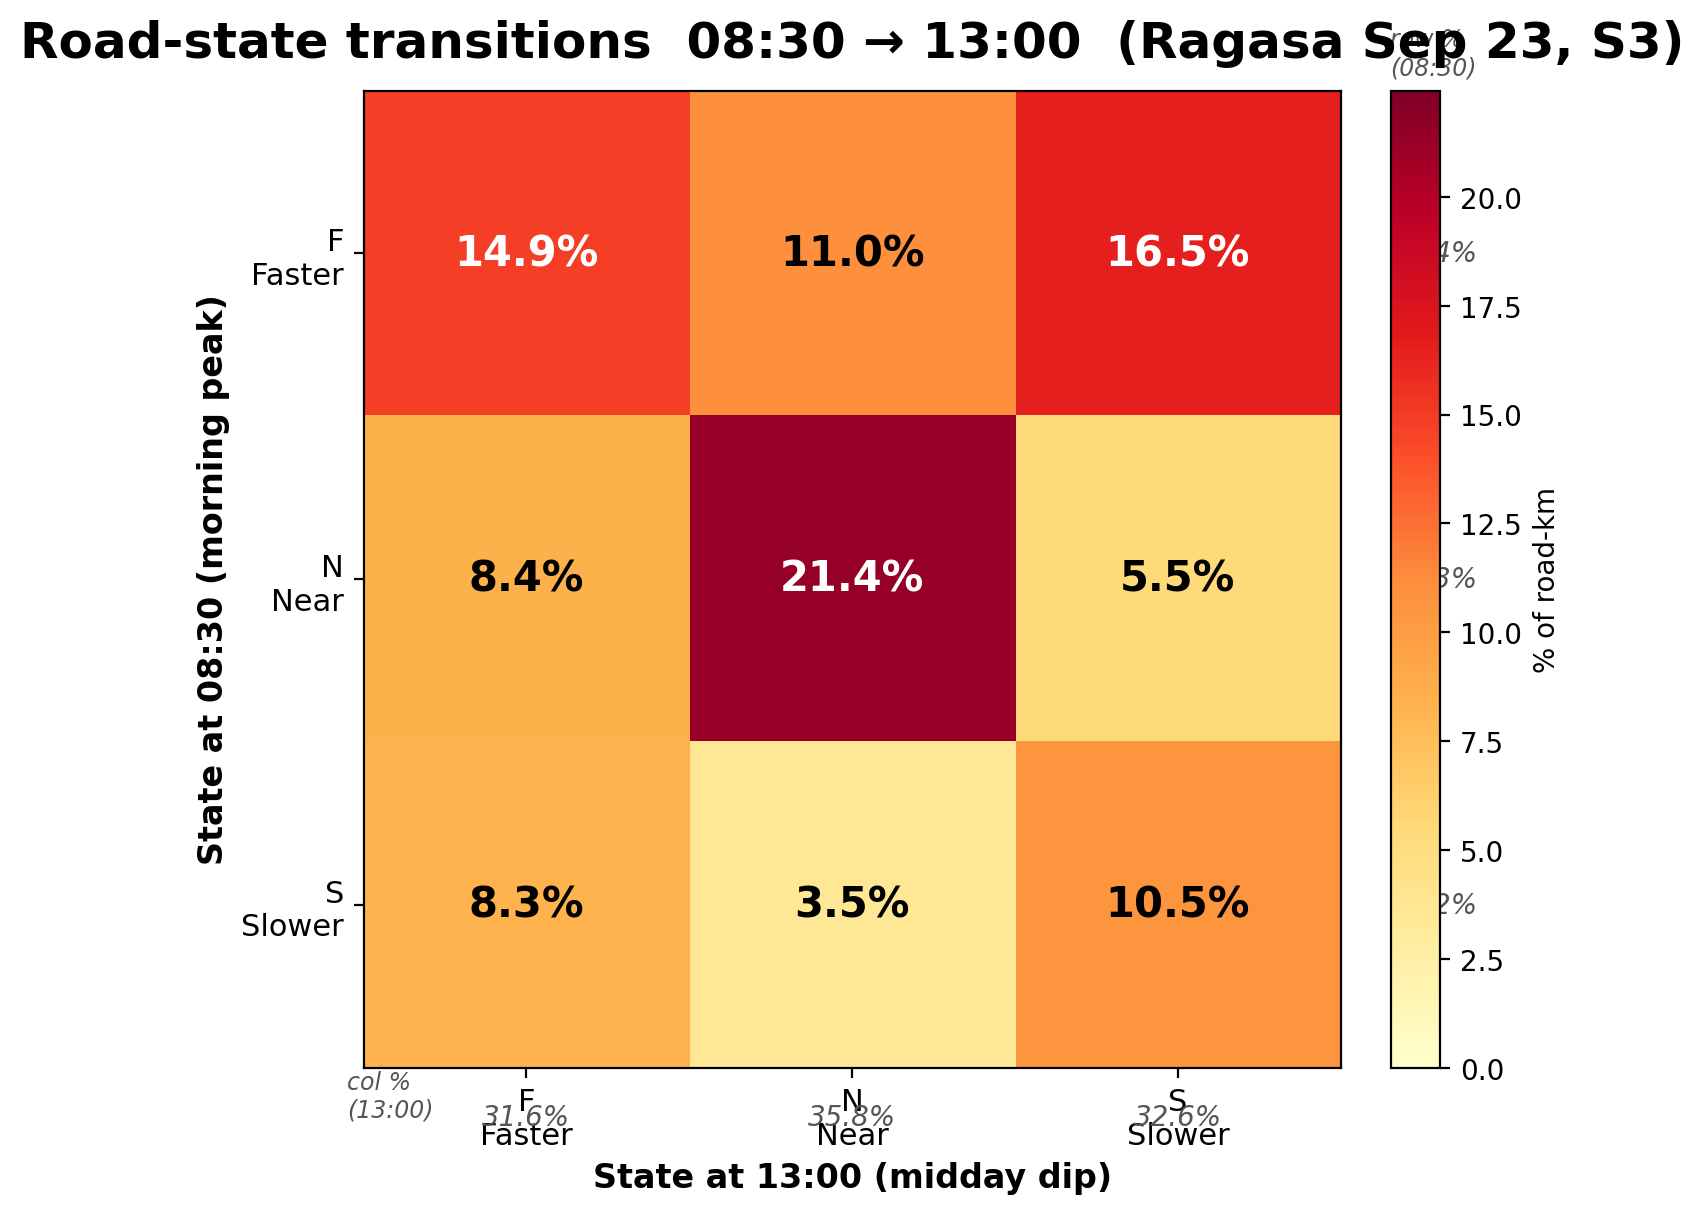
\includegraphics[width=0.85\linewidth]{图50f_transition_matrix.png}
\caption{Length-weighted state transition matrix 08:30 $\rightarrow$ 13:00 (Ragasa, Sep 23, Signal 3).}
\end{figure}

\section{Cox PH analysis plan (planned future work)}
The Cox proportional hazards model proposed in Chapter 7 will use the following specification:
\begin{equation}
h_i(t) = h_0(t) \, \exp\!\big(\beta_1 \mathrm{Cat}_i + \beta_2 \mathrm{BCQ}_i + \beta_3 X_i^{\mathrm{built}} + \beta_4 X_i^{\mathrm{incident}} + \beta_5 \mathrm{Coast}_i\big),
\end{equation}
where $\mathrm{Cat}_i$ is a road-category dummy vector, $\mathrm{BCQ}_i$ is the baseline-congestion quintile, $X_i^{\mathrm{built}}$ collects employment-resident ratio, retail and tourism density, $X_i^{\mathrm{incident}}$ is the during-event incident count within 500\,m, and $\mathrm{Coast}_i$ is distance to coast. The recovery time is hours from the S8$\rightarrow$S3 downgrade until two consecutive slots within $|\Delta RS| \le 0.03$; roads not recovered by the end of the observation window are right-censored. Proportional hazards assumptions will be tested using scaled Schoenfeld residuals.

\chapter{Data Processing Notes}

\section{Data ingestion}
The primary input is the TomTom Traffic Index 30-minute relative-speed feed for September--October 2025. Each 30-minute snapshot is delivered as a parquet file with one row per road segment containing: road category, road subcategory, left-hand-traffic flag, road-closure flag, relative speed in $[0,1]$, and a WKB binary geometry. Snapshots are organised under \texttt{data/flow\_parquet2/YYYY-MM-DD/slotNN.parquet}, where \texttt{slotNN} indexes the 30-minute slot of the day (00--47). Incident data is stored separately under \texttt{data/incident\_parquet/} with two-level date/hour partitioning, and is joined to road segments by spatial proximity (within 500\,m of segment centroid).

\section{Road registry construction}
TomTom does not provide a stable road identifier across snapshots, so a road registry is built by extracting all unique WKB geometries observed across the full data range. Two-level identifiers are produced. The \texttt{road\_id} is a hash of the exact WKB string; the \texttt{cluster\_id} groups WKB variants that share the same start and end coordinates (endpoint clustering) into a single physical road. Endpoint clustering is used because TomTom emits slightly different vertex sequences for the same physical segment across snapshots: the average physical road has 6.9 WKB variants. The endpoint clustering produces 95,167 physical roads from 166,159 raw WKBs.

\section{Baseline construction}
Each typhoon observation is matched against a baseline observation for the same physical road, the same 30-minute slot-of-day, and the same day type. Day types are: WORKDAY (Mon--Fri excluding 2025-10-01 and 2025-10-07 public holidays), SATURDAY, and SUNDAY-HOLIDAY. The choice to keep Saturday as a separate type is data-driven: the three day-type speed curves differ in shape, with Saturday showing a flatter morning peak than Sunday/holiday. Baseline aggregates are computed only over non-typhoon days in the observation window (excluding 09-17 through 09-20, 09-22 through 09-25, 10-03 through 10-05, and 10-10). The baseline table contains 1,677,503 (cluster $\times$ day-type $\times$ slot) cells.

When multiple WKB variants of the same physical road appear in the same slot, their relative speeds are averaged before being written to the baseline. Observations with \texttt{road\_closure = 1} are excluded from baseline aggregates but are retained in typhoon-period analysis.

\section{Handling missing data}
Data coverage is incomplete on several days. The most severe gap is on 2025-09-22, when 32 of 48 slots are missing entirely (during the Ragasa Signal 1 phase). 09-14 is missing 19 slots after 14:30, 09-15 is sparsely missing 24 scattered slots, and 09-16 is missing slot 04. Missing snapshots are treated as missing observations rather than as zero traffic. Roads with fewer than three observed days in the matching baseline are flagged as unreliable and excluded from regression analyses. Baseline reliability tiers based on the number of observed days are: $n \ge 5$ in 14.5\% of cells, $n \ge 3$ in 30.3\%, and $n \ge 1$ in all 100\%.

\section{Slot-level aggregation and grid joins}
For grid-level analyses, road centroids are joined to a 500\,m hexagonal grid covering the Hong Kong land area. Built-environment covariates from OpenStreetMap (schools, retail, tourism, transport, medical, recreation POIs) and demographic data are pre-aggregated to the hex grid and then attached to roads by centroid lookup. The OSM extracts are cached locally under \texttt{data/osm\_cache/} to keep grid construction reproducible.

\section{Reproducibility and code organisation}
The analysis pipeline is split into numbered Python scripts. Three are foundational: \texttt{build\_road\_registry.py} produces the WKB-to-road-id map; \texttt{cluster\_roads.py} adds endpoint cluster identifiers; \texttt{compute\_baseline.py} produces the baseline table. The remaining analysis scripts (numbered 01 through 67 in the project directory) consume these outputs and emit figures and CSV tables one phase at a time. Each script is self-contained and can be re-run independently; intermediate outputs are versioned by filename.

\section{Known caveats}
Three caveats apply to all results. First, the 09-22 coverage gap means the Ragasa pre-event analysis effectively starts from Signal 3 rather than Signal 1. Second, the \texttt{road\_closure} attribute uses \texttt{NaN} to indicate ``not closed'' rather than \texttt{0}; filters in derived scripts use \texttt{road\_closure != 1} accordingly. Third, the \texttt{wkb\_hash} field in early registry versions used the Python built-in \texttt{hash()}, which is not stable across processes; downstream joins now use endpoint-key matching (\texttt{ep\_key}) rather than \texttt{wkb\_hash} to avoid this hazard.

\end{document}
